%definira klasu dokumenta 
\documentclass[12pt]{report} 

%prostor izmedu naredbi \documentclass i \begin{document} se zove uvod. U njemu se nalaze naredbe koje se odnose na cijeli dokument

%osnovni LaTex ne može riješiti sve probleme, pa se koriste različiti paketi koji olakšavaju izradu željenog dokumenta
\usepackage[croatian]{babel} 
\usepackage{amssymb}
\usepackage{amsmath}
\usepackage{txfonts}
\usepackage{mathdots}
\usepackage{titlesec}
\usepackage{array}
\usepackage{lastpage}
\usepackage{etoolbox}
\usepackage{tabularray}
\usepackage{color, colortbl}
\usepackage{adjustbox}
\usepackage{geometry}
\usepackage[classicReIm]{kpfonts}
\usepackage{hyperref}
\usepackage{fancyhdr}

\usepackage{float}
\usepackage{setspace}
\restylefloat{table}


\patchcmd{\chapter}{\thispagestyle{plain}}{\thispagestyle{fancy}}{}{} %redefiniranje stila stranice u paketu fancyhdr

%oblik naslova poglavlja
\titleformat{\chapter}{\normalfont\huge\bfseries}{\thechapter.}{20pt}{\Huge}
\titlespacing{\chapter}{0pt}{0pt}{40pt}


\linespread{1.3} %razmak između redaka

\geometry{a4paper, left=1in, top=1in,}  %oblik stranice

\hypersetup{ colorlinks, citecolor=black, filecolor=black, linkcolor=black,	urlcolor=black }   %izgled poveznice


%prored smanjen između redaka u nabrajanjima i popisima
\newenvironment{packed_enum}{
	\begin{enumerate}
		\setlength{\itemsep}{0pt}
		\setlength{\parskip}{0pt}
		\setlength{\parsep}{0pt}
	}{\end{enumerate}}

\newenvironment{packed_item}{
	\begin{itemize}
		\setlength{\itemsep}{0pt}
		\setlength{\parskip}{0pt}
		\setlength{\parsep}{0pt}
	}{\end{itemize}}




%boja za privatni i udaljeni kljuc u tablicama
\definecolor{LightBlue}{rgb}{0.9,0.9,1}
\definecolor{LightGreen}{rgb}{0.9,1,0.9}

%Promjena teksta za dugačke tablice
\DefTblrTemplate{contfoot-text}{normal}{Nastavljeno na idućoj stranici}
\SetTblrTemplate{contfoot-text}{normal}
\DefTblrTemplate{conthead-text}{normal}{(Nastavljeno)}
\SetTblrTemplate{conthead-text}{normal}
\DefTblrTemplate{middlehead,lasthead}{normal}{Nastavljeno od prethodne stranice}
\SetTblrTemplate{middlehead,lasthead}{normal}

%podesavanje zaglavlja i podnožja

\pagestyle{fancy}
\lhead{Programsko inženjerstvo}
\rhead{FlipMemo}
\lfoot{CanonPrinter}
\cfoot{stranica \thepage/\pageref{LastPage}}
\rfoot{\today}
\renewcommand{\headrulewidth}{0.2pt}
\renewcommand{\footrulewidth}{0.2pt}


\begin{document} 
	
	
	
	\begin{titlepage}
		\begin{center}
			\vspace*{\stretch{1.0}} %u kombinaciji s ostalim \vspace naredbama definira razmak između redaka teksta
			\LARGE Programsko inženjerstvo\\
			\large Ak. god. 2023./2024.\\
			
			\vspace*{\stretch{3.0}}
			
			\huge FlipMemo\\
			\Large Dokumentacija, Rev. \textit{$<$1 ili 2$>$}\\
			
			\vspace*{\stretch{12.0}}
			\normalsize
			Grupa: \textit{CanonPrinter}\\
			Voditelj: \textit{Jurica Runtas}\\
			
			
			\vspace*{\stretch{1.0}}
			Datum predaje: \textit{$<$dan$>$. $<$mjesec$>$. $<$godina$>$.}\\
	
			\vspace*{\stretch{4.0}}
			
			Nastavnik: \textit{$<$Ime i prezime nastavnika zaduženog za vašu grupu$>$}\\
		
		\end{center}

	
	\end{titlepage}

	
	\tableofcontents


	\chapter{Dnevnik promjena dokumentacije}
		
		\begin{longtblr}[
				label=none
			]{
				width = \textwidth, 
				colspec={|X[2]|X[13]|X[3]|X[3]|}, 
				rowhead = 1
			}
			\hline
			\textbf{Rev.}	& \textbf{Opis promjene/dodatka} & \textbf{Autori} & \textbf{Datum}\\[3pt] \hline
			0.1 & Napravljen predložak. \newline Upisane osnovne informacije o timu. & Jurica Runtas & 22.10.2023. \\[3pt] \hline 
			0.2	& Dodani dionici, aktori i njihovi funkcionalni zahtjevi. & Jurica Runtas & 25.10.2023. 	\\[3pt] \hline 
			0.2.1 & Opis projekta i ostali zahtjevi. & Jan Kuzman & 30.10.2023. \\[3pt] \hline 
			0.3 & Opisi obrazaca uporabe & Lovro Švenda & 27.10.2023. \\[3pt] \hline 
			0.3.1 & Dodani dijagrami obrasca uporabe, izmjena opisa obrasca uporabe & Kristijan Milić & 29.10.2023. \\[3pt] \hline 
			0.3.2 & Uređen format opisa obrazaca uporabe i napravljene manje izmjene & Jurica Runtas & 29.10.2023. \\[3pt] \hline 
			0.4 & Sekvencijski dijagrami & Matej Galić & 30.10.2023. \\[3pt] \hline
			0.4.1 & Napravljeni prvi i drugi sekvencijski dijagrami & Matej Galić & 30.10.2023. \\[3pt] \hline
			0.4.2 & Napravljeni treći i četvrti sekvencijski dijagrami & Josip Ćurić & 30.10.2023. \\[3pt] \hline
			0.5 & Arhitektura i dizajn sustava & Lovro Švenda & 4.11.2023. \\[3pt] \hline
			0.5.1 & Dodani dijagrami razreda & Kristijan Milić & 5.11.2023. \\[3pt] \hline
			0.5.2 & Uređeni dijagrami razreda, dodane veze na dijagramu DTO-a & Jurica Runtas & 5.11.2023. \\[3pt] \hline
			0.5.3 & Opis arhitekture baze podataka & Josip Ćurić & 7.11.2023. \\[3pt] \hline
			0.5.4 & Opis dijagrama razreda & Lovro Švenda & 17.11.2023. \\[3pt] \hline
			1.0 & Konačna verzija dokumentacije za prvu predaju & Jurica Runtas & 17.11.2023 \\ [3pt]
			\hline
			1.1 & Dijagram razmještaja & Jurica Runtas & 3.1.2024 \\ [3pt]
			\hline
			1.2 & Upute za puštanje u pogon & Jurica Runtas & 4.1.2024 \\ [3pt]
			\hline
			1.3 & Korištene tehnologije i alati & Jurica Runtas & 4.1.2024 \\ [3pt]
			\hline
			1.4 & Ispitivanje komponenti & Jurica Runtas & 7.1.2024 \\ [3pt]
			\hline
			1.5 & Ispitivanje sustava & Jurica Runtas & 8.1.2024 \\ [3pt]
			\hline
			1.6 & Dijagram stanja i dijagram aktivnosti & Josip Ćurić & 12.1.2024 \\ [3pt]
			\hline
			1.7 & Zaključak i budući rad & Jan Kuzman & 13.1.2024 \\ [3pt] \hline
			1.8 & Dijagram komponenti & Kristijan Milić & 17.1.2024 \\ [3pt] \hline
			1.9 & Dijagram razreda & Lovro Švenda & 19.1.2024. \\ [3pt] \hline
			2.0 & Konačna verzija dokumentacije za drugu predaju & Jurica Runtas & 19.1.2024. \\ [3pt] \hline
		\end{longtblr}
	\chapter{Opis projektnog zadatka}
		
Cilj ovog projekta je razviti aplikaciju za učenje stranog jezika koja se bazira na ponavljanju s odmakom (još i poznato pod „spaced repetition“). Popularne aplikacije kao što su Quizlet, Anki te Memrise. Nove riječi se uče postavljanjem pitanja o riječima koje su prethodno definirane u bazi riječi. Učenik odgovara s prijevodima riječi odabirući ispravan odabir od nekoliko ponuđenih alternativnih riječi. Ako učenik točno odgovori na pitanje, riječ koja se nalazi u pitanju se pomiče u sljedeću skupinu/posudu riječi, no ako učenik netočno odgovori na pitanje, riječ će se vratiti na „početak“ odnosno u prvu skupinu/posudu riječi koje se smatraju ne naučenima. Svaka skupina, koje su međusobno povezane u niz, ima određeno vrijeme „trajanja“ prema čijem isteku riječ postaje ponovno dostupna za prikazivanje učeniku u formi pitanja. Vrijeme trajanja za prvu skupinu koja se nalazi u nizu je jedan dan, druga skupina u nizu ima vrijeme trajanja od 2 dana te se za svaku sljedeću skupinu broj dana udvostručuje. Aplikacija ima        broj posuda te ako se riječ nalazi u posljednjoj od povezanih posuda, tada se po isteku vremena riječ smatra naučenom te se smješta u posebnu posudu i više ne sudjeluje u učenju strane riječi. 

Administrator dodaje strane riječi, iz odabranog stranog jezika, u aplikaciju. Uzmimo za primjer engleski jezik kako bi pokazali funkcionalnost aplikacije. Svaka riječ koja će se učiti se sastoji od engleske riječi, opisa riječi koji je sačinjen od nekoliko fraza ili rečenica, prijevoda engleske riječi na hrvatski te nekoliko rečenica/fraza koje je bolje opisuju te na posljetku glasovne datoteke izgovora na engleskom jeziku. Svaka riječ koja je dodana u bazu se može obrisati ili joj se mogu promijeniti komponente. Riječi su povezane u rječnike koji se sastoje od imena i riječi. Nove riječi se mogu dodati u jedan ili više otprije postojanih rječnika. Kod definiranja riječi, administrator riječi ima pomoć u obliku savjeta koji su prikupljeni od strane vanjskog izbora. Aplikacija komunicira s vanjskim rječnikom (https://rapidapi.com/collection/thesaurus-apis) kada administrator upiše dio riječi te pokrene proceduru pretrage preko koje se prihvaćaju riječi i njezini opisi. 

Učenik/korisnik se može registrirati putem elektroničke pošte i promijeniti lozinku. Prilikom prvog login-a se na korisnikovu elektroničku poštu šalje privremena lozinka koja se mora promijeniti. 
Atributi korisničkog/učeničkog računa: 
1.	Elektronička pošta 
2.	Lozinka 
Učenik odabire jedan od ponuđenih rječnika te može pokrenuti učenje riječi. 
Učenje riječi se može odvijati kroz nekoliko različitih mode-ova
Mode-ovi:
1.	Upit engleske riječi uz odabir hrvatskog prijevoda 
2.	Upit hrvatske riječi uz odabir engleskog prijevoda
3.	Upit izgovorom engleske riječi uz pisanje riječi na engleskom (provjera ispravnog pisanja)
4.	Upit tekstualnim oblikom engleske riječi uz snimanje izgovora u zvučnu datoteku
Netočni odgovori ponuđeni studentu se izabiru slučajnim odabirom iz skupine odgovora koji moraju biti istog tipa drugih rječnika kod mode-ova učenja gdje se prezentira više opcija odabira. Za kontrolu snimljenih datoteka u kojima su izgovorene riječi stranog jezika „postoji“ servis koji kontrolira točnost izgovorenih riječi i vraća povratnu ocjenu. Implementirano je i umjetno aplikacijsko sučelje koje će prihvatiti takvu glasovnu datoteku te će povratno vratiti ocjenu na ljestvici od 1 do 10. 

Bez obzira koji jezik učili, funkcionalnosti su jednako implementirane za sve jezike. Svaki rječnik ima dodatnu oznaku kako bi se znalo na koji jezik se on odnosi te sadrži riječi samo jednog jezika. Rječnici su grupirani po jeziku te se takvi prikazuju učeniku/korisniku prilikom odabira rječnika. 

Hijerarhijski postoji glavni administrator sa najvećim ovlastima koje su mu korijenski dodijeljene. On može druge korisničke/učeničke račune „unaprijediti“ u administratore koji će imati jednake ovlasti kao i on sam. Učenički računi ne ovise o administratorskim te se oni sami registriraju i brišu svoj korisnički račun po potrebi.

Za kraj opisa projekta proći ćemo kroz aplikaciju po imenu Quizlet, ranije navedenu, te ćemo pogledati njihov način implementacije.

\begin{figure}[H]
	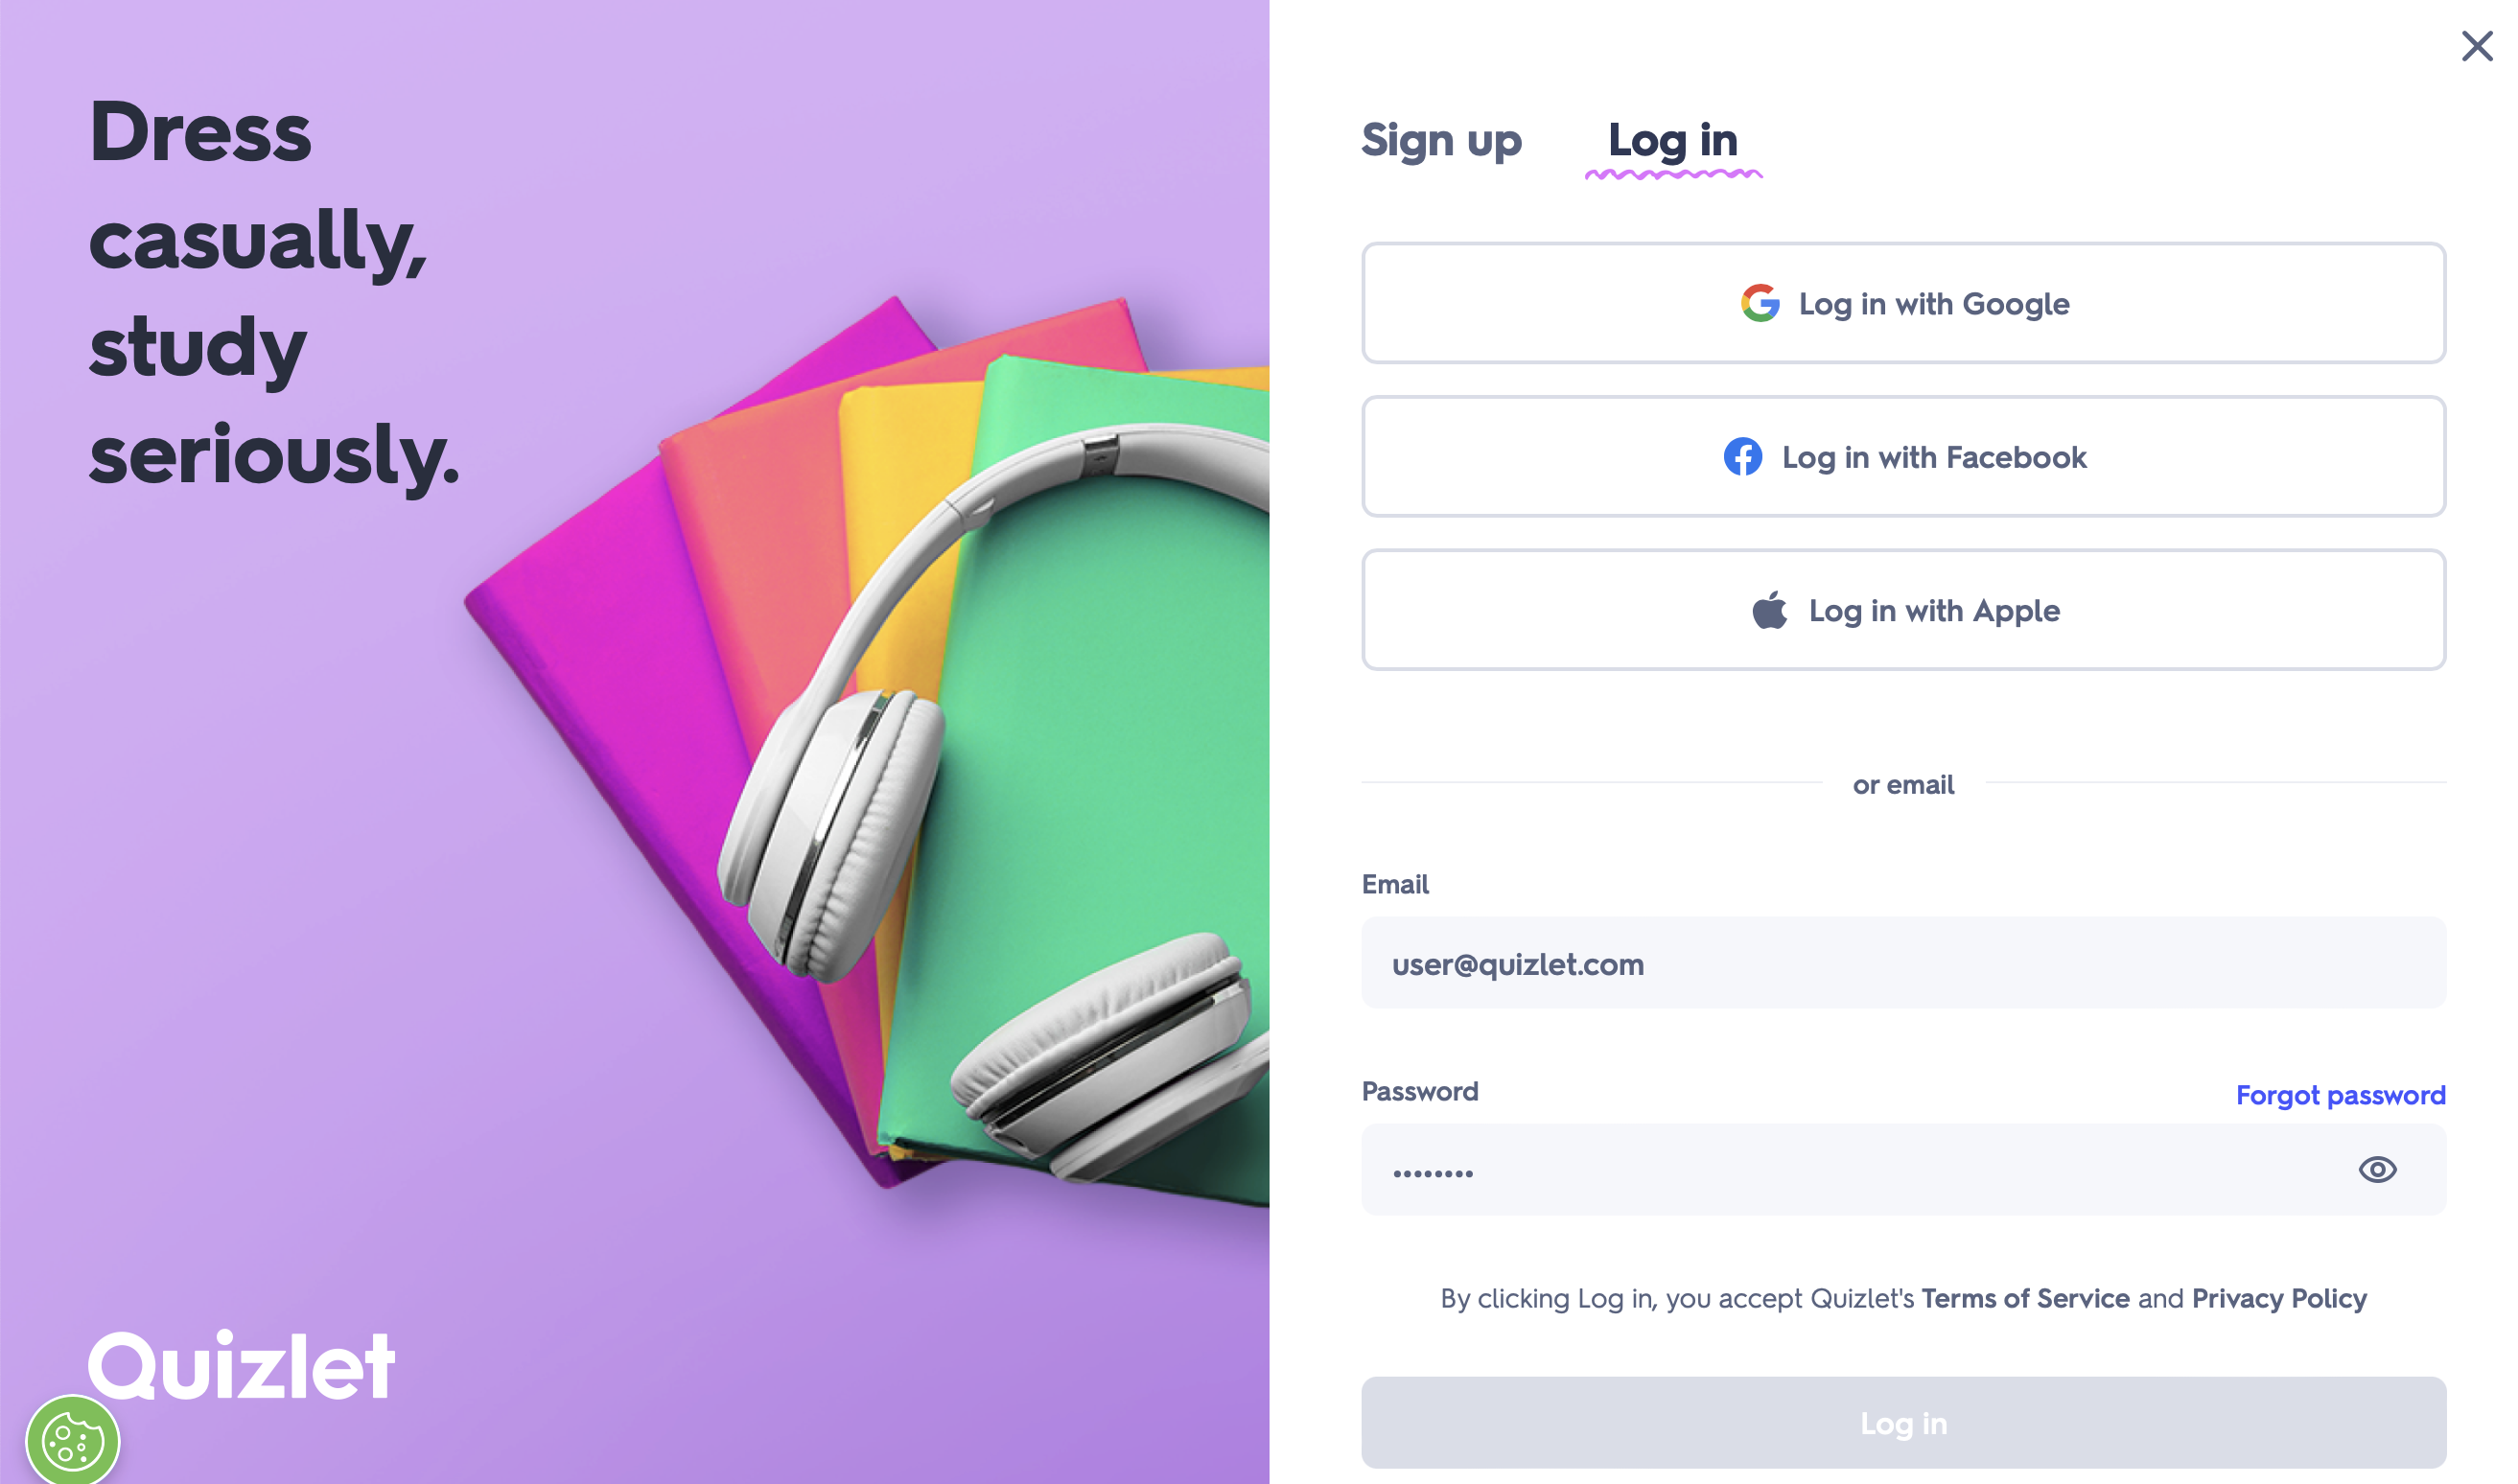
\includegraphics[width=\textwidth]{SlikeOpisProjekta/login_screen_quizlet.png} %veličina u odnosu na širinu linije
	\caption{Slika login stranice Quizeta}
	\label{fig:LoginScreenQuizlet} %label mora biti drugaciji za svaku sliku
\end{figure}

		\eject
		
		\section{Primjeri u \LaTeX u}
		
		\textit{Ovo potpoglavlje izbrisati.}\\

		U nastavku se nalaze različiti primjeri kako koristiti osnovne funkcionalnosti \LaTeX a koje su potrebne za izradu dokumentacije. Za dodatnu pomoć obratiti se asistentu na projektu ili potražiti upute na sljedećim web sjedištima:
		\begin{itemize}
			\item Upute za izradu diplomskog rada u \LaTeX u - \url{https://www.fer.unizg.hr/_download/repository/LaTeX-upute.pdf}
			\item \LaTeX\ projekt - \url{https://www.latex-project.org/help/}
			\item StackExchange za Tex - \url{https://tex.stackexchange.com/}\\
		
		\end{itemize} 	


		
		\noindent \underbar{podcrtani tekst}, \textbf{podebljani tekst}, 	\textit{nagnuti tekst}\\
		\noindent \normalsize primjer \large primjer \Large primjer \LARGE {primjer} \huge {primjer} \Huge primjer \normalsize
				
		\begin{packed_item}
			
			\item  primjer
			\item  primjer
			\item  primjer
			\item[] \begin{packed_enum}
				\item primjer
				\item[] \begin{packed_enum}
					\item[1.a] primjer
					\item[b] primjer
				\end{packed_enum}
				\item primjer
			\end{packed_enum}
			
		\end{packed_item}
		
		\noindent primjer url-a: \url{https://www.fer.unizg.hr/predmet/proinz/projekt}
		
		\noindent posebni znakovi: \# \$ \% \& \{ \} \_ 
		$|$ $<$ $>$ 
		\^{} 
		\~{} 
		$\backslash$ 
		
		
		\begin{longtblr}[
			label=none,
			entry=none
			]{
				width = \textwidth,
				colspec={|X[8,l]|X[8, l]|X[16, l]|}, 
				rowhead = 1,
			} %definicija širine tablice, širine stupaca, poravnanje i broja redaka naslova tablice
			\hline \SetCell[c=3]{c}{\textbf{naslov unutar tablice}}	 \\ \hline[3pt]
			\SetCell{LightGreen}IDKorisnik & INT	&  	Lorem ipsum dolor sit amet, consectetur adipiscing elit, sed do eiusmod  	\\ \hline
			korisnickoIme	& VARCHAR &   	\\ \hline 
			email & VARCHAR &   \\ \hline 
			ime & VARCHAR	&  		\\ \hline 
			\SetCell{LightBlue} primjer	& VARCHAR &   	\\ \hline 
		\end{longtblr}
		

		\begin{longtblr}[
				caption = {Naslov s referencom izvan tablice},
				entry = {Short Caption},
			]{
				width = \textwidth, 
				colspec = {|X[8,l]|X[8,l]|X[16,l]|}, 
				rowhead = 1,
			}
			\hline
			\SetCell{LightGreen}IDKorisnik & INT	&  	Lorem ipsum dolor sit amet, consectetur adipiscing elit, sed do eiusmod  	\\ \hline
			korisnickoIme	& VARCHAR &   	\\ \hline 
			email & VARCHAR &   \\ \hline 
			ime & VARCHAR	&  		\\ \hline 
			\SetCell{LightBlue} primjer	& VARCHAR &   	\\ \hline 
		\end{longtblr}
	


		
		
		%unos slike
		\begin{figure}[H]
			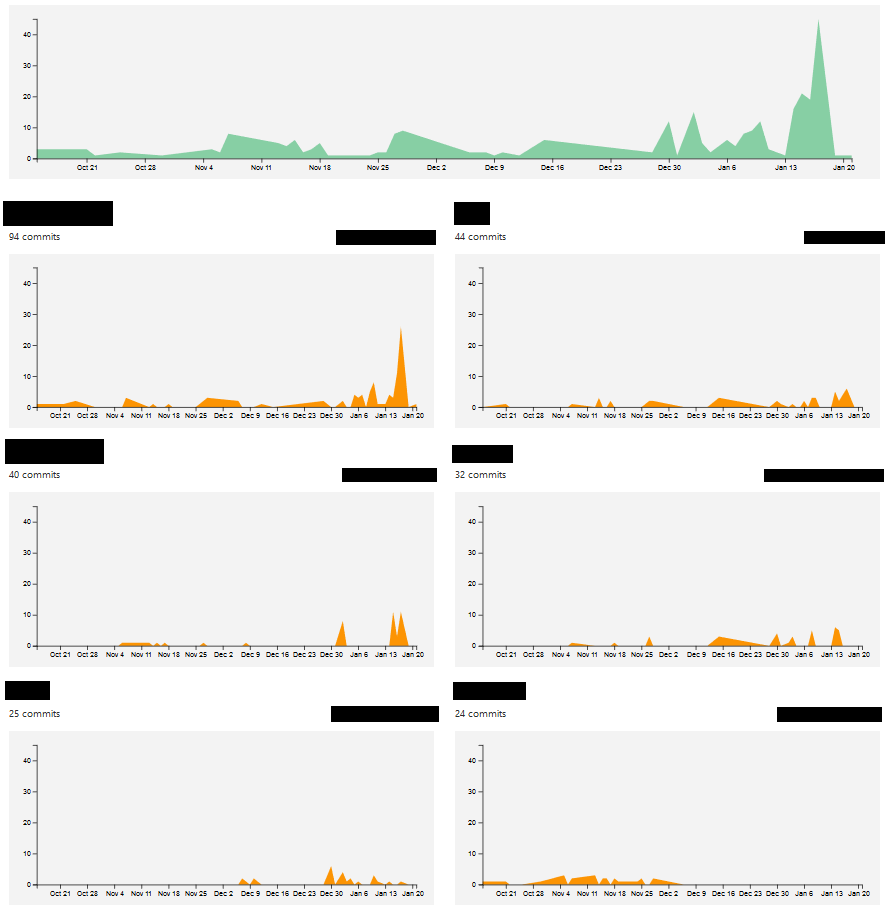
\includegraphics[scale=0.4]{slike/aktivnost.PNG} %veličina slike u odnosu na originalnu datoteku i pozicija slike
			\centering
			\caption{Primjer slike s potpisom}
			\label{fig:promjene}
		\end{figure}
		
		\begin{figure}[H]
			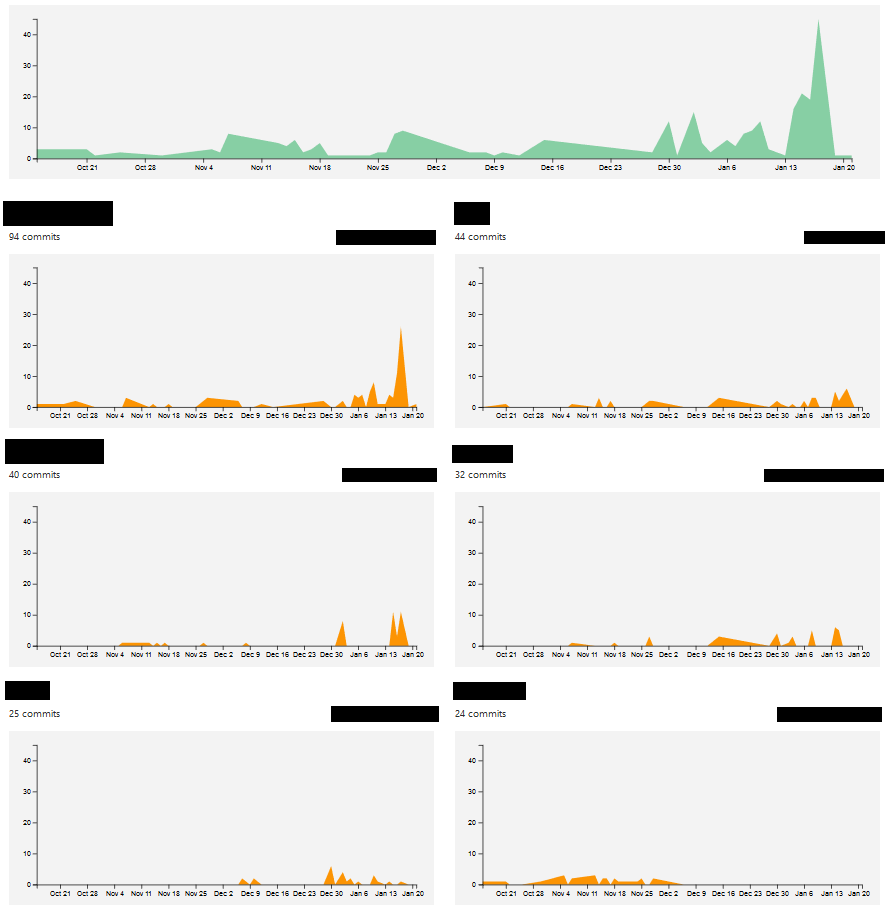
\includegraphics[width=\textwidth]{slike/aktivnost.PNG} %veličina u odnosu na širinu linije
			\caption{Primjer slike s potpisom 2}
			\label{fig:promjene2} %label mora biti drugaciji za svaku sliku
		\end{figure}
		
		Referenciranje slike \ref{fig:promjene2} u tekstu.
		
		\eject
		
	
	\chapter{Specifikacija programske potpore}
		
	\section{Funkcionalni zahtjevi}
			
			\noindent \textbf{Dionici:}
			
			\begin{packed_enum}
				
				\item Naručitelji
				\item Učenici (korisnici)
				\item Administratori				
				\item Razvojni tim
				
			\end{packed_enum}
			
			\noindent \textbf{Aktori i njihovi funkcionalni zahtjevi:}
			
			
			\begin{packed_enum}
				\item  \underbar{Neregistrirani učenik (inicijator) može:}
				
				\begin{packed_enum}
					
					\item se registrirati e-mail adresom
					
				\end{packed_enum}
			
			
				\item  \underbar{Učenik (inicijator) može:}
				
				\begin{packed_enum}
					\item izvršiti prijavu u sustav za koju su mu potrebni e-mail adresa i lozinka
					\item promijeniti trenutnu lozinku
					\item obrisati svoj korisnički račun
					\item pregledavati postojeće rječnike grupirane po jeziku
					\item pokrenuti učenje riječi odabirom jednog od ponuđenih rječnika i načina učenja
					\item odgovarati na pitanja o riječima ovisno o odabranom načinu učenja
					
					\begin{packed_enum}
						\item odabirom točnog odgovora
						\item upisivanjem točnog odgovora
						\item snimanjem izgovora riječi u zvučnu datoteku
					\end{packed_enum}
					
				\end{packed_enum}
			
					
			\item  \underbar{Administrator (inicijator) može:}
			
			\begin{packed_enum}
				
				\item stvarati nove rječnike
				\item dodavati i brisati riječi iz rječnika
				\item uređivati komponente postojećih riječi u rječniku\newline
				
			\end{packed_enum}
			
			
			\item  \underbar{Korijenski administrator (inicijator) može:}
			
			\begin{packed_enum}
				
				\item definirati administratore
				\item stvarati nove rječnike
				\item dodavati i brisati riječi iz rječnika
				\item uređivati komponente postojećih riječi u rječniku
				
			\end{packed_enum}
		
			
			\item  \underbar{Baza podataka (sudionik):}
		
			\begin{packed_enum}
			
			\item pohranjuje rječnike
			\item pohranjuje sve podatke o učenicima i administratorima
			
			\end{packed_enum}
		
			
			\item  \underbar{Vanjski rječnik (sudionik):}
		
			\begin{packed_enum}
			
			\item sadrži informacije koje se koriste prilikom dodavanja novih riječi u rječnike
			
			\end{packed_enum}
		
			
			\item  \underbar{Servis za ocjenu kvalitete izgovora (sudionik):}
	
			\begin{packed_enum}
		
			\item provjerava točnost snimljene izgovorene riječi
			\item na temelju provjere odgovara s ocjenom u ljestvici od jedan do deset
		
			\end{packed_enum}		
		
	
			\end{packed_enum}
			
			\eject 
			
						
			\subsection{Obrasci uporabe}
					
				\subsubsection{Opis obrazaca uporabe}		

					\noindent \underbar{\textbf{UC1 - Registracija}}
					\begin{packed_item}
	
						\item \textbf{Glavni sudionik: }Učenik
						\item  \textbf{Cilj:} Stvoriti korisnički račun za pristup sustavu
						\item  \textbf{Sudionici:} Baza podataka
						\item  \textbf{Preduvjet:} -
						\item  \textbf{Opis osnovnog tijeka:}
						
						\item[] \begin{packed_enum}
	
							\item Učenik odabire gumb za registraciju
							\item Učenik unosi potrebne korisničke podatke
							\item Učenik prima obavijest o uspješnoj registraciji
						\end{packed_enum}
						
						\item  \textbf{Opis mogućih odstupanja:}
						
						\item[] \begin{packed_item}
	
							\item[2.a] Unos već zauzetog e-maila, unos već zauzetog korisničkog imena, unos neispravnog e-maila
							\item[] \begin{packed_enum}
								
								\item Sustav obavještava učenika o neuspjeloj registraciji i vraća ga natrag na stranicu za registraciju
								\item Učenik mijenja potrebne unesene podatke i završava unos ili odustaje od registracije
								
							\end{packed_enum}
							
						\end{packed_item}
					\end{packed_item}

					\noindent \underbar{\textbf{UC2 - Prijava u sustav}}
					\begin{packed_item}
	
						\item \textbf{Glavni sudionik: }Učenik
						\item  \textbf{Cilj:} Izvršiti prijavu u sustav
						\item  \textbf{Sudionici:} Baza podataka
						\item  \textbf{Preduvjet:} Registracija
						\item  \textbf{Opis osnovnog tijeka:}
						
						\item[] \begin{packed_enum}
	
							\item Unos korisničkog imena ili e-maila i lozinke
							\item Potvrda o ispravnosti unesenih podataka
							\item Pristup korisničkom sučelju
						\end{packed_enum}
						
						\item  \textbf{Opis mogućih odstupanja:}
						
						\item[] \begin{packed_item}
	
							\item[2.a] Neispravno uneseno korisničko ime, email ili lozinka
							\item[] \begin{packed_enum}
								
								\item Sustav obavještava učenika o neuspjeloj prijavi te ga vraća na stranicu za prijavu
								
							\end{packed_enum}
							
						\end{packed_item}
					\end{packed_item}

					\noindent \underbar{\textbf{UC3 - Pregled osobnih podataka}}
					\begin{packed_item}
	
						\item \textbf{Glavni sudionik: }Učenik
						\item  \textbf{Cilj:} Pregledati osobne podatke
						\item  \textbf{Sudionici:} Baza podataka
						\item  \textbf{Preduvjet:} Učenik je prijavljen u sustav
						\item  \textbf{Opis osnovnog tijeka:}
						
						\item[] \begin{packed_enum}
	
							\item Učenik odlazi na svoj profil
							\item Učenik odabire opciju "Osobni podatci"
							\item Aplikacije prikazuje osobne podatke učenika
						\end{packed_enum}
						
					\end{packed_item}

					\noindent \underbar{\textbf{UC4 - Promjena osobnih podataka}}
					\begin{packed_item}
	
						\item \textbf{Glavni sudionik: }Učenik
						\item  \textbf{Cilj:} Promijeniti osobne podatke
						\item  \textbf{Sudionici:} Baza podataka
						\item  \textbf{Preduvjet:} Učenik je prijavljen u sustav
						\item  \textbf{Opis osnovnog tijeka:}
						
						\item[] \begin{packed_enum}
	
							\item Učenik odlazi na svoj profil
							\item Učenik bira koje osobne podatke želi mijenjati
							\item Učenik mijenja odabrane osobne podatke
							\item Učenik sprema promjene
							\item Baza podataka ažurira napravljene promjene
						\end{packed_enum}
						
						\item  \textbf{Opis mogućih odstupanja:}
						
						\item[] \begin{packed_item}
	
							\item[4.a] Učenik mijenja svoje podatke, ali ne spremi promjene
							\item[] \begin{packed_enum}
								
								\item Sustav obavještava učenika da nije spremio podatke
								\item Učenik odabire želi li spremiti ili odbaciti napravljene promjene 
								
							\end{packed_enum}
							
						\end{packed_item}
					\end{packed_item}

					\noindent \underbar{\textbf{UC5 - Brisanje korisničkog računa}}
					\begin{packed_item}
	
						\item \textbf{Glavni sudionik: }Učenik
						\item  \textbf{Cilj:} Izbrisati svoj korisnički račun
						\item  \textbf{Sudionici:} Baza podataka
						\item  \textbf{Preduvjet:} Učenik je prijavljen u sustav
						\item  \textbf{Opis osnovnog tijeka:}
						
						\item[] \begin{packed_enum}
	
							\item Učenik odlazi na svoj profil
							\item Učenik bira opciju obriši korisnički račun
							\item Sustav ispituje učenika je li siguran da želi obrisati korisnički račun
							\item Učenik potvrđuje da želi obrisati korisnički račun
							\item Korisnički račun se briše iz baze podataka
							\item Sustav šalje učenika na stranicu za registraciju
						\end{packed_enum}
						
						\item  \textbf{Opis mogućih odstupanja:}
						
						\item[] \begin{packed_item}
	
							\item[4.a] Učenik ne potvrđuje brisanje računa, a izlazi iz aplikacije
							\item[] \begin{packed_enum}
								
								\item Sustav ne briše korisnički račun i obavještava učenika da korisnički račun nije obrisan
								
							\end{packed_enum}
							
						\end{packed_item}
					\end{packed_item}

					\noindent \underbar{\textbf{UC6 - Pregled rječnika}}
					\begin{packed_item}
	
						\item \textbf{Glavni sudionik: }Učenik
						\item  \textbf{Cilj:} Pregledati postojeće rječnike za učenje
						\item  \textbf{Sudionici:} Baza podataka
						\item  \textbf{Preduvjet:} Učenik je prijavljen u sustav
						\item  \textbf{Opis osnovnog tijeka:}
						
						\item[] \begin{packed_enum}
	
							\item Učenik odabire opciju "Pregled rječnika"
							\item Otvara se padajuća lista dostupnih jezika
							\item Učenik odabire jezik
							\item Otvara se stranica sa izborom rječnika koji su dostupni na odabranom jeziku
							\item Učenik odabire rječnik
							\item Otvara se stranica na kojoj učenik može pregledavati rječnik
						\end{packed_enum}
						
					\end{packed_item}

					\noindent \underbar{\textbf{UC7 - Pokretanje učenja}}
					\begin{packed_item}
	
						\item \textbf{Glavni sudionik: }Učenik
						\item  \textbf{Cilj:} Pokrenuti učenje jezika
						\item  \textbf{Sudionici:} Baza podataka
						\item  \textbf{Preduvjet:} Učenik je prijavljen u sustav
						\item  \textbf{Opis osnovnog tijeka:}
						
						\item[] \begin{packed_enum}
	
							\item Učenik bira opciju "Pokreni učenje"
							\item Otvara se padajuća lista jezika rječnika
							\item Učenik odabire jezik
							\item Otvara se stranica sa izborom rječnika koji dostupni na odabranom jeziku
							\item Učenik odabire rječnik iz kojeg želi učiti
							\item Otvara se stranica sa ponuđenim načinima učenja
							\item Učenik odabire način na koji želi učiti jezik
							\item Otvara se stranica na kojoj učenik odgovara na pitanja o riječima na temelju načina učenja kojeg je odabrao
						\end{packed_enum}
						
					\end{packed_item}

					\noindent \underbar{\textbf{UC8 - Prekid učenja}}
					\begin{packed_item}
	
						\item \textbf{Glavni sudionik: }Učenik
						\item  \textbf{Cilj:} Prekinuti učenje i spremiti napredak
						\item  \textbf{Sudionici:} Baza podataka
						\item  \textbf{Preduvjet:} Učenik je prijavljen u sustav
						\item  \textbf{Opis osnovnog tijeka:}
						
						\item[] \begin{packed_enum}
	
							\item Učenik bira opciju "Prekini učenje"
							\item U bazu podataka se sprema napredak koji je učenik napravio na određenom rječniku, jeziku i načinu učenja
							\item Sustav učenika vraća na početnu stranicu aplikacije
						\end{packed_enum}
						
					\end{packed_item}

					\noindent \underbar{\textbf{UC9 - Promjena načina učenja}}
					\begin{packed_item}
	
						\item \textbf{Glavni sudionik: }Učenik
						\item  \textbf{Cilj:} Promijeniti način na koji učenik uči određeni jezik
						\item  \textbf{Sudionici:} Baza podataka
						\item  \textbf{Preduvjet:} Učenik je prijavljen u sustav
						\item  \textbf{Opis osnovnog tijeka:}
						
						\item[] \begin{packed_enum}
	
							\item Učenik bira opciju "Promijeni način učenja"
							\item Otvara se stranica sa jezicima
							\item Učenik odabire jezik koji trenutno uči
							\item Otvara se stranica sa izborom rječnika
							\item Učenik odabire rječnik iz kojeg trenutno uči
							\item Otvara se stranica sa ponuđenim načinima učenja
							\item Učenik odabire način na koji želi učiti jezik
							\item Baza podataka ažurira način učenja za određeni rječnik i jezik
						\end{packed_enum}
						
					\end{packed_item}

					\noindent \underbar{\textbf{UC10 - Učenje po odabranom načinu učenja}}
					\begin{packed_item}
	
						\item \textbf{Glavni sudionik: }Učenik
						\item  \textbf{Cilj:} Učiti jezik na način koji je učenik odabrao
						\item  \textbf{Sudionici:} Baza podataka
						\item  \textbf{Preduvjet:} Učenik je pokrenuo proces učenja
						\item  \textbf{Opis osnovnog tijeka:}
						
						\item[] \begin{packed_enum}
	
							\item Učeniku se postavlja pitanje o odabranoj riječi ovisno o načinu učenja, podatcima o učenju i odabranom rječniku
							\item Učeniku se nudi obrazac za odgovor na postavljeno pitanje
							\item Učenik obrascem odgovara na postavljeno pitanje
							\item Učenik potvrđuje svoj odgovor na obrascu
							\item Baza podataka ažurira podatke učenja učenika određenim rječnikom, jezikom i načinom učenja
							\item Ponavlja se prvi korak sve dok učenik ne prekine učenje
						\end{packed_enum}

						\item  \textbf{Opis mogućih odstupanja:}
						
						\item[] \begin{packed_item}
	
							\item[5.a] Nije moguće spajanje na bazu podataka
							\item[] \begin{packed_enum}
								
								\item Učenik dobiva informaciju o nedostupnosti baze podataka i prekida se učenje
								
							\end{packed_enum}
						\end{packed_item}
						
					\end{packed_item}

					\noindent \underbar{\textbf{UC11 - Dodavanje administratora}}
					\begin{packed_item}
	
						\item \textbf{Glavni sudionik: }Korijenski administrator
						\item  \textbf{Cilj:} Definirati nove administratore
						\item  \textbf{Sudionici:} Baza podataka
						\item  \textbf{Preduvjet:} Korisnik je prijavljen u sustav i dodijeljena su mu prava korijenskog administratora
						\item  \textbf{Opis osnovnog tijeka:}
						
						\item[] \begin{packed_enum}
	
							\item Korijenski administator odabire opciju postavljanja administratora
							\item Otvara se prozor za upis korisničkog imena korisnika
							\item Korijenski administrator upisuje korisničko ime i potvrđuje upis
							\item Baza podataka ažurira promjene za određeno korisničko ime
						\end{packed_enum}

						\item  \textbf{Opis mogućih odstupanja:}
						
						\item[] \begin{packed_item}
	
							\item[3.a] Upisano je neispravno korisničko ime
							\item[] \begin{packed_enum}
								
								\item Sustav obavještava korijenskog administratora o neuspjelom upisu
								
							\end{packed_enum}
						\end{packed_item}
						
					\end{packed_item}

					\noindent \underbar{\textbf{UC12 - Stvori rječnik}}
					\begin{packed_item}
	
						\item \textbf{Glavni sudionik: }Administrator
						\item  \textbf{Cilj:} Stvoriti novi rječnik
						\item  \textbf{Sudionici:} Baza podataka, Vanjski rječnik
						\item  \textbf{Preduvjet:} Korisnik je prijavljen u sustav i dodijeljena su mu prava administratora
						\item  \textbf{Opis osnovnog tijeka:}
						
						\item[] \begin{packed_enum}
	
							\item Administrator odabire opciju "Stvori novi rječnik"
							\item Administrator unosi riječi i podatke o novom rječniku
							\item Baza podataka ažurira novi rječnik
						\end{packed_enum}
						
					\end{packed_item}

					\noindent \underbar{\textbf{UC13 - Dodaj riječ}}
					\begin{packed_item}
	
						\item \textbf{Glavni sudionik: }Administrator
						\item  \textbf{Cilj:} Dodati riječ u postojeći rječnik
						\item  \textbf{Sudionici:} Baza podataka, Vanjski rječnik
						\item  \textbf{Preduvjet:} Korisnik je prijavljen u sustav i dodijeljena su mu prava administratora
						\item  \textbf{Opis osnovnog tijeka:}
						
						\item[] \begin{packed_enum}
	
							\item Administrator odabire opciju "Dodaj novu riječ"
							\item Otvara se prozor za odabir jezika i rječnika
							\item Administrator odabire jezik i rječnik u koji želi dodati novu riječ
							\item Otvara se prozor za upis riječi
							\item Administrator upisuje riječ
							\item Pokreće se procedura pretrage na vanjskom rječniku
							\item Administrator odabire opis i ostale podatke bitne za riječ koje je dobio od vanjskog rječnika
							\item Administrator uređuje odabrane podatke
							\item Administrator potvrđuje unos
							\item Baza podataka ažurira novu riječ za određeni jezik i rječnik
					
						\end{packed_enum}

						\item  \textbf{Opis mogućih odstupanja:}
						
						\item[] \begin{packed_item}
	
							\item[5.a] Upisana riječ već postoji u rječniku
							\item[] \begin{packed_enum}
								
								\item Sustav obavještava administratora o tome da upisana riječ već postoji u rječniku
								\item Administrator može odabrati opciju uređivanja postojeće riječi ili upisati drugu riječ
								
							\end{packed_enum}
						\end{packed_item}
						
					\end{packed_item}

					\noindent \underbar{\textbf{UC14 - Ukloni riječ}}
					\begin{packed_item}
	
						\item \textbf{Glavni sudionik: }Administrator
						\item  \textbf{Cilj:} Ukloniti riječ iz rječnika
						\item  \textbf{Sudionici:} Baza podataka
						\item  \textbf{Preduvjet:} Korisnik je prijavljen u sustav i dodijeljena su mu prava administratora
						\item  \textbf{Opis osnovnog tijeka:}
						
						\item[] \begin{packed_enum}
	
							\item Administrator odabire opciju "Ukloni riječ"
							\item Otvara se prozor za odabir jezika i rječnika
							\item Administrator odabire jezik i rječnik iz kojeg želi ukloniti riječ
							\item Otvara se prozor za upis riječi
							\item Administrator upisuje riječ
							\item Odabrana riječ se briše iz rječnika
						\end{packed_enum}

						\item  \textbf{Opis mogućih odstupanja:}
						
						\item[] \begin{packed_item}
	
							\item[5.a] Upisana riječ ne postoji
							\item[] \begin{packed_enum}
								
								\item Sustav obavještava administratora da upisana riječ ne postoji u rječniku
							\end{packed_enum}
						\end{packed_item}
						
					\end{packed_item}

					\noindent \underbar{\textbf{UC15 - Izmijeni riječ}}
					\begin{packed_item}
	
						\item \textbf{Glavni sudionik: }Administrator
						\item  \textbf{Cilj:} Izmijeniti riječ iz rječnika
						\item  \textbf{Sudionici:} Baza podataka
						\item  \textbf{Preduvjet:} Korisnik je prijavljen u sustav i dodijeljena su mu prava administratora
						\item  \textbf{Opis osnovnog tijeka:}
						
						\item[] \begin{packed_enum}
	
							\item Administrator odabire opciju "Izmijeni riječ"
							\item Otvara se prozor za odabir jezika i rječnika
							\item Administrator odabire jezik i rječnik u kojem želi izmijeniti riječ
							\item Otvara se prozor za upis riječi
							\item Administrator upisuje riječ
							\item Otvara se prozor za izmjenu opisa i podataka riječi
							\item Administrator mijenja opis riječi i podatke o riječi
							\item Administrator sprema promjene
							\item Baza podataka ažurira određenu riječ za određeni jezik i rječnik
						\end{packed_enum}

						\item  \textbf{Opis mogućih odstupanja:}
						
						\item[] \begin{packed_item}
	
							\item[5.a] Upisana riječ ne postoji
							\item[] \begin{packed_enum}
								
								\item Sustav obavještava administratora da upisana riječ ne postoji u rječniku
								
							\end{packed_enum}
							\item[8.a] Administrator nije spremio promjene
							\item[] \begin{packed_enum}
								
								\item Sustav obavještava administratora da nije spremio promjene
								\item Administrator odlučuje želi li spremiti ili odbaciti napravljene promjene
								
							\end{packed_enum}

						\end{packed_item}			
					\end{packed_item}
				
					
				\subsubsection{Dijagrami obrazaca uporabe}
					
					\begin{figure}[H]
						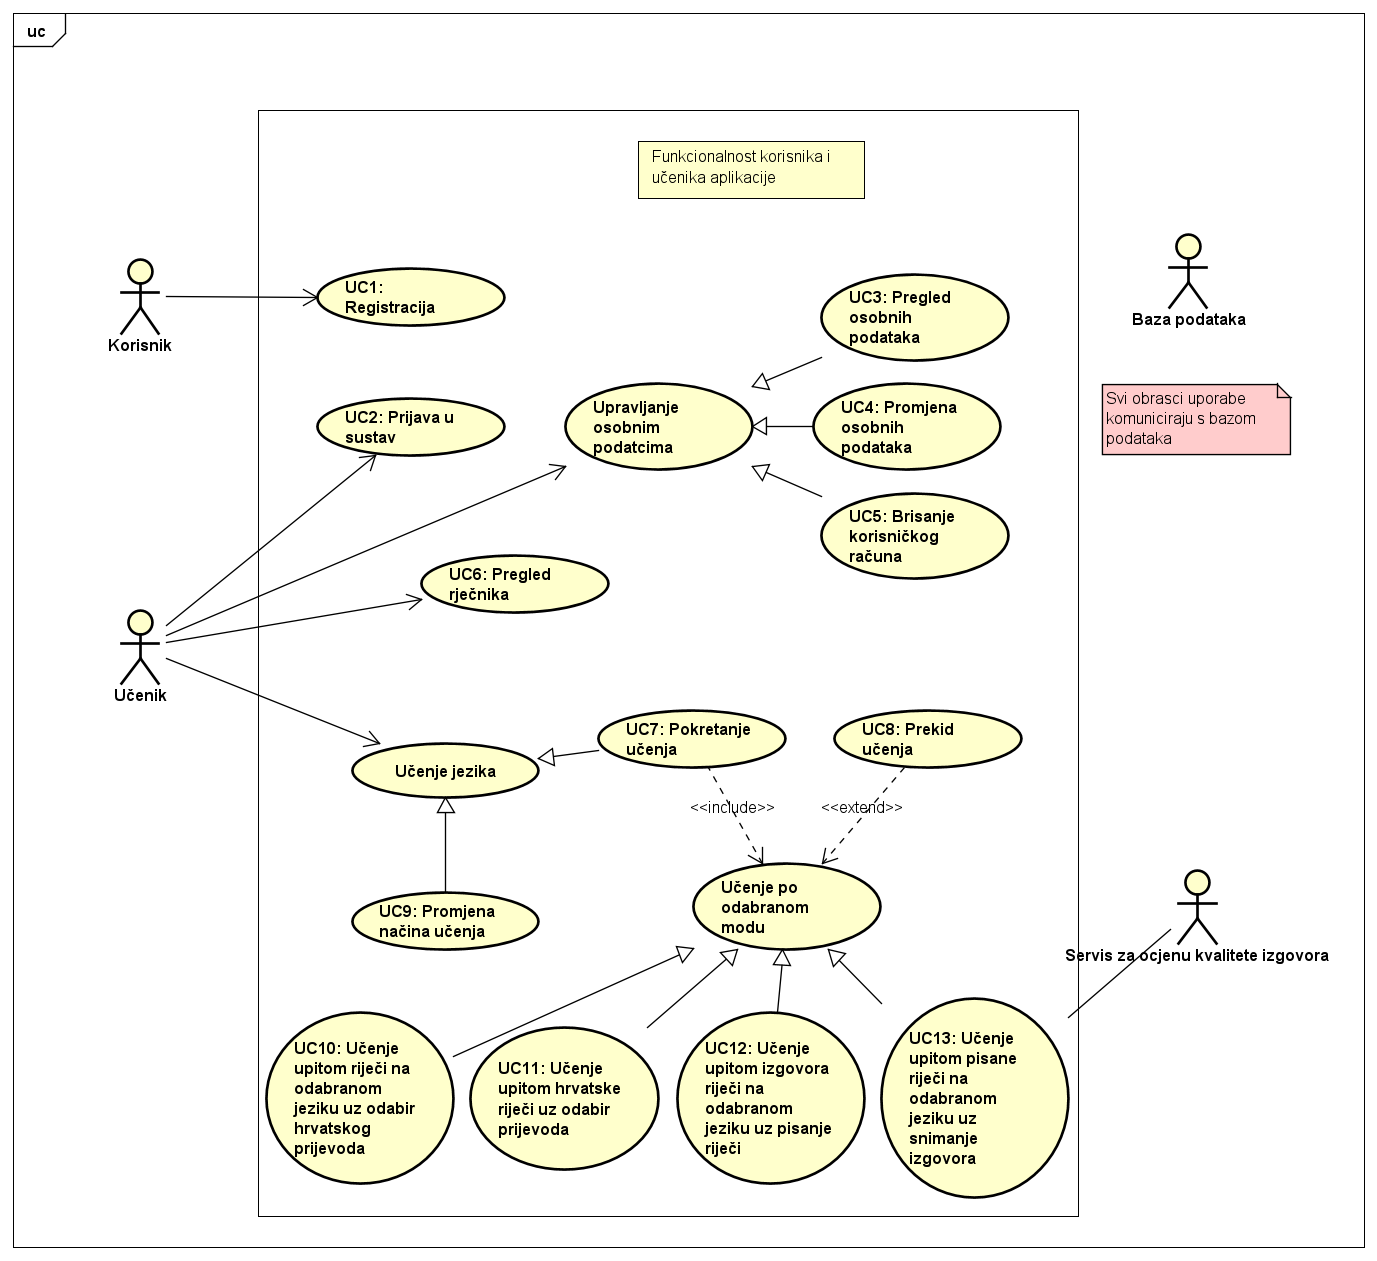
\includegraphics[width=\textwidth]{dijagrami/ucdiag1.png} %veličina u odnosu na širinu linije
						\caption{Dijagram obrasca uporabe, funkcionalnost korisnika i učenika}
						\label{fig:ucdiag1} %label mora biti drugaciji za svaku sliku
					\end{figure}

					\begin{figure}[H]
						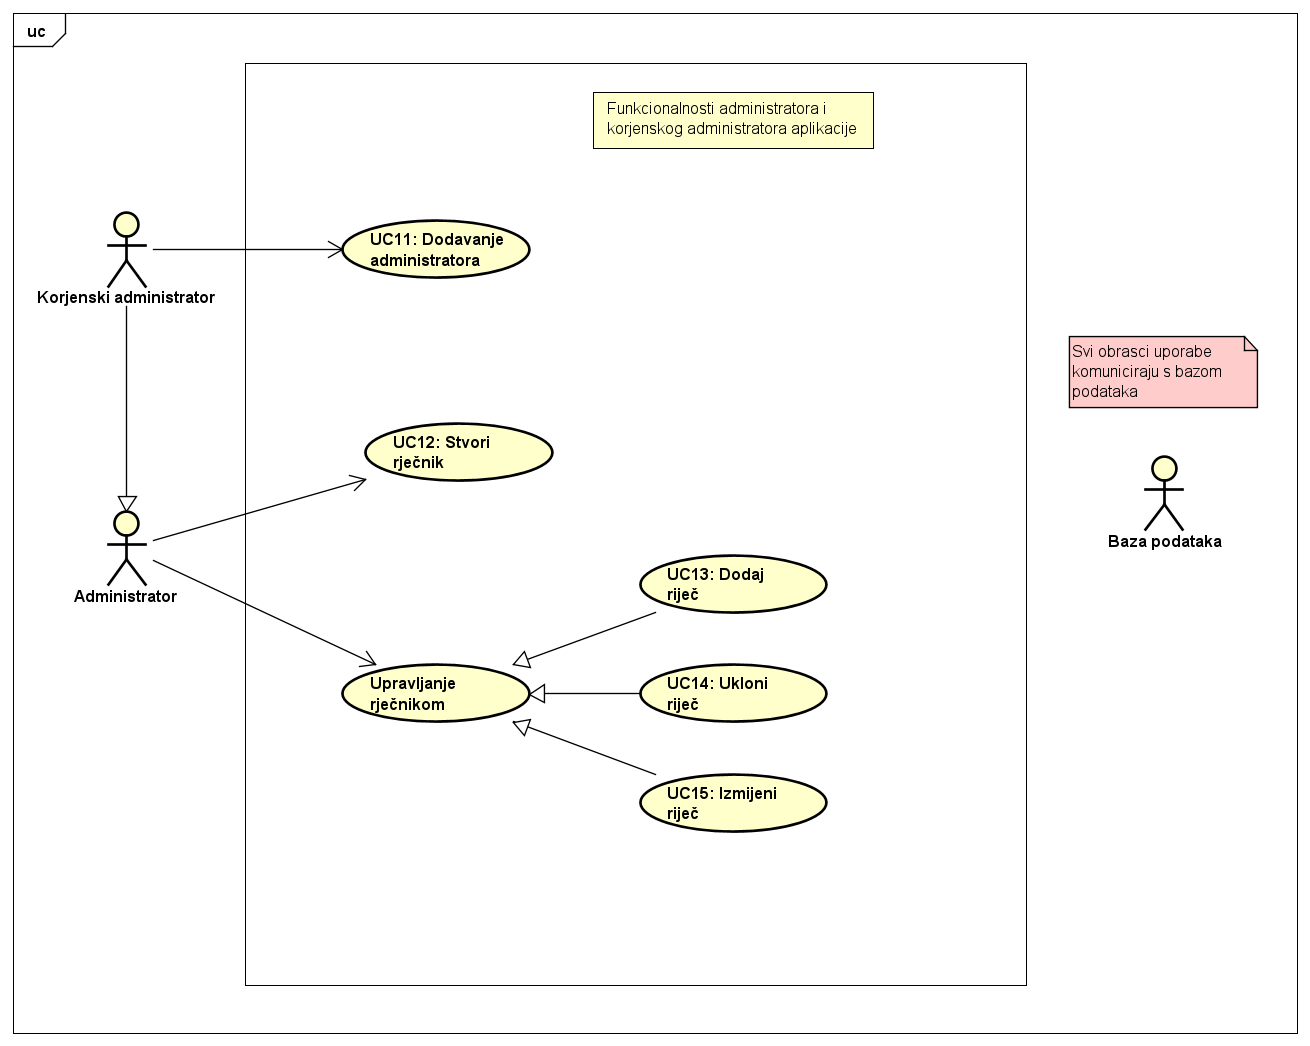
\includegraphics[width=\textwidth]{dijagrami/ucdiag2.png} %veličina u odnosu na širinu linije
						\caption{Dijagram obrasca uporabe, funkcionalnost korijenskog administratora i administratora}
						\label{fig:ucdiag2} %label mora biti drugaciji za svaku sliku
					\end{figure}

				\eject		
				
			\subsection{Sekvencijski dijagrami}
				
				\textbf{\textit{dio 1. revizije}}\\
				
				\textit{Nacrtati sekvencijske dijagrame koji modeliraju najvažnije dijelove sustava (max. 4 dijagrama). Ukoliko postoji nedoumica oko odabira, razjasniti s asistentom. Uz svaki dijagram napisati detaljni opis dijagrama.}
				\eject
	
		\section{Ostali zahtjevi}
		
			\textbf{\textit{dio 1. revizije}}\\
		 
			 \textit{Nefunkcionalni zahtjevi i zahtjevi domene primjene dopunjuju funkcionalne zahtjeve. Oni opisuju \textbf{kako se sustav treba ponašati} i koja \textbf{ograničenja} treba poštivati (performanse, korisničko iskustvo, pouzdanost, standardi kvalitete, sigurnost...). Primjeri takvih zahtjeva u Vašem projektu mogu biti: podržani jezici korisničkog sučelja, vrijeme odziva, najveći mogući podržani broj korisnika, podržane web/mobilne platforme, razina zaštite (protokoli komunikacije, kriptiranje...)... Svaki takav zahtjev potrebno je navesti u jednoj ili dvije rečenice.}
			 
			 
			 
	
	\chapter{Arhitektura i dizajn sustava}

		\text{Arhitektura aplikacije može se podijeliti na 3 podsustava:}
	\begin{itemize}
		\item 	\text{Web preglednik}
		\item 	\text{Web poslužitelj/Web aplikacija}
		\item 	\text{Baza podataka}		
	\end{itemize}

	\begin{figure}[H]
		\centering
		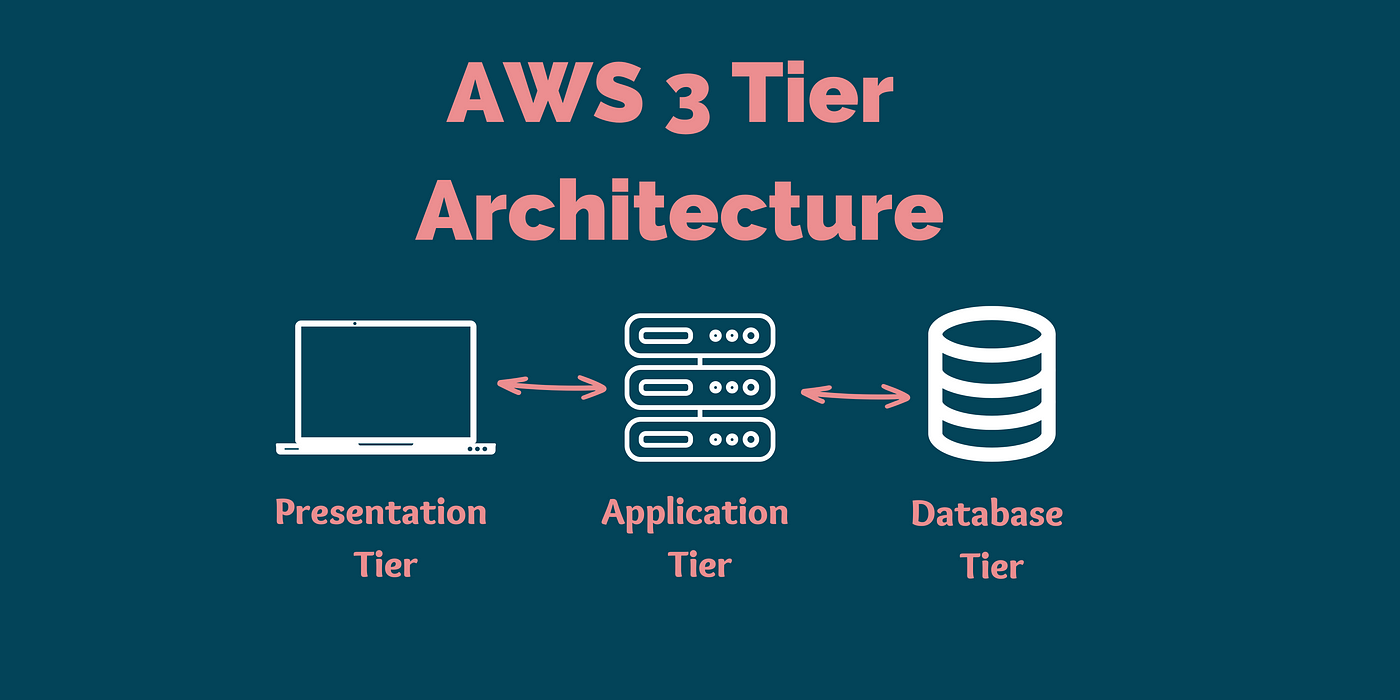
\includegraphics[width=100mm]{slike/arhitektura.png}
		\caption{Arhitektura sustava}
		\label{fig:arhitektura}
	\end{figure}

	\indent{\textit{\underline{Web preglednik}} je program koji korisniku omogućuje pregled
	web-stranica i multimedijalnih sadržaja vezanih uz njih. Svaki web preglednik je predvoditelj korištenja web aplikacija,
	jer omogućuje korisniku da preko web preglednika šalje zahtjeve web poslužitelju.}

	\indent{\textit{\underline{Web poslužitelj}} je osnova rada web aplikacije. On pokreće cijeli sustav rada aplikacije
	te joj prosljeđuje zahtjeve od korisnika. Osnovna zadaća web poslužitelja je omogućiti komunikaciju između korisnika i aplikacije, a ta
	komunikacija se odvija preko HTTP protokola. To je vrsta protokola koja se koristi za prijenos informacija na internetu.}

	\indent{\textit{\underline{Web aplikacija}} je dio web poslužitelja koja služi korisniku za obradu željenih zahtjeva.
	Web aplikacija radi tako da prima zahtjeve i ovisno o zahtjevu pristupa {\textit{\underline{bazi podataka}}} iz koje dohvaća
	"odgovore" na željene zahtjeve. Te "odgovore" šalje natrag korisniku preko web poslužitelja u obliku HTML dokumenta kojeg
	korisnik vidi u web pregledniku.}

	\indent{Programski jezik kojeg smo odabrali za izradu naše web aplikacije je Python. U sklopu Pythona koristimo Django, radni okvir koji služi za izradu web aplikacija. Razvojno okruženje koje koristimo
	je Microsoft Visual Studio Code. Arhitektura sustava temelji se na MVC odnosno MTV konceptu.}

	\indent{Django je modeliran oko MVC arhitekture, no svoju arhitekturu definira kao MTV (eng. {\textit{Model-Template-View}})
	arhitekturu. Komponentu upravitelj (eng. {\textit{Controller}}) zamjenjuje komponentom pogled (eng. {\textit{View}}) te
	komponentu pogled s komponentom predložak (eng. {\textit{Template}}). MTV razdvaja različite dijelove web-stranice: prikaz,
	pristup podatcima i logiku web stranice. Također omogućava neovisnu izgradnju web-stranica, povećava sigurnost sustava te
	pojednostavljuje održavanje sustava.}

	\noindent{MTV se sastoji od:}
	\begin{itemize}
		\item 	\textbf{Model} - definira oblike i odnose podataka u bazi podataka. Model u Django okruženju je klasa napisana
				u programskom jeziku Python. Određuje varijable i metode pridužene određenim tipovima podataka te ima značenje
				tablice u bazi podataka. Model je usko povezan s bazom podataka i pogledom. Od baze podataka model dohvaća tražene
				podatke i prosljeđuje ih pogledu.
		\item 	\textbf{Predložak} - sloj arhitekture MTV-a usko povezan s web-preglednikom. Predložak je HTML stranica s dodanim
				strukturama koje omogućavaju prikaz podataka koji su proslijeđeni od pogleda. Zadaća predloška je sadržaj primljen
				od pogleda organizirati i ugraditi u HTML kod koji će se prikazati u web-pregledniku.
		\item 	\textbf{Pogled} - određuje koji će podatci biti prikazani, odnosno, koji će podatci biti dohvaćeni iz baze podataka
				i prikazani pomoću predloška u web-pregledniku. U Djangu prilikom stvaranja nove web-aplikacije za svaku pojedinu
				aplikaciju stvara se zasebna datoteka pogleda. Pogled ne zna kako su podatci prikazani u web-pregledniku. Posao
				pogleda je dohvatiti tražene podatke i proslijediti ih višem sloju koji će ih prikazati u pregledniku.
	\end{itemize}
	
		

		

				
		\section{Baza podataka}
			
		{Potrebe sustava za bazu podataka su relativno jednostavne, a relacije između entiteta nisu osobito kompleksne. Zbog tih razloga, sustav za bazu podataka koristi MongoDB – \textit{NoSQL}, dokumentno-orijentiranu bazu podataka.} \\ {Entiteti za pohranjivanje podataka su:}
		\begin{itemize}
			\item 	\textbf{Word}{,}
			\item 	\textbf{PronunciationAudio}{,}
			\item 	\textbf{Dictionary}{,}
			\item 	\textbf{Account}{.}
			\item 	\textbf{WordProgress}{,}
			\item 	\textbf{DictionaryProgress}{.}
		\end{itemize}
		{Zvučni zapis izgovora riječi odvojen je od same riječi na koju se odnosi jer je zvučna datoteka relativno veća od ostatka podataka za riječ čime se ubrzava vrijeme dohvata riječi kada se ne koristi način učenja slovkanjem riječi uz dani izgovor.}
		
			\subsection{Opis tablica}
			

				\textit{Važno je istaknuti da je svakom MongoDB dokumentu automatski pridodjeljen , uz ostale atribute, jedinstveni ObjectId u "\_id" atributu (primarni ključ) te je on u tablicama prikazan samo ondje gdje se eksplicitno koristi.} \\
				
				\textbf{Word} \\ {Opisuje riječ. Više rječnika može sadržavati iste riječi pa je veza \textit{N..N}. Sadrži strani ključ na zvučni zapis izgovora riječi na ciljanom jeziku. Veza sa zvučnim zapisom je \textit{N..1}. Svi dokumenti entiteta \textbf{Word} sadržani su u kolekciji "Words".}
				
				\begin{longtblr}[
					label=none,
					entry=none
					]{
						width = \textwidth,
						colspec={|X[8,l]|X[6, l]|X[20, l]|}, 
						rowhead = 1,
					} %definicija širine tablice, širine stupaca, poravnanje i broja redaka naslova tablice
					\hline \SetCell[c=3]{c}{\textbf{Word}}	 \\ \hline[3pt]
					\SetCell{LightGreen}\_id & objectId	&  	Primarni ključ riječi.  	\\ \hline
					word & string	&  	Zapis riječi na ciljanom jeziku.  	\\ \hline
					translation	& string &   Prevedeni zapis riječi na hrvatskom.	\\ \hline 
					descriptionLang & string	&  	Opis riječi na ciljanom jeziku.	\\ \hline
					descriptionCro & string	&  	Opis riječi na hrvatskome jeziku.	\\ \hline  
					\SetCell{LightBlue} audio\_id	& objectId &   Primarni ključ zvučnog zapisa izgovora riječi na ciljanom jeziku.	\\ \hline 
				\end{longtblr}
				
				\textbf{PronunciationAudio} \\ {Sadrži zvučni zapis izgovora na ciljanom jeziku nekih riječi. Veza s riječima je \textit{1..N} u slučaju postojanja homofona. Svi dokumenti entiteta \textbf{PronunciationAudio} sadržani su u kolekciji "PronunciationAudios".}
				
				\begin{longtblr}[
					label=none,
					entry=none
					]{
						width = \textwidth,
						colspec={|X[8,l]|X[6, l]|X[20, l]|}, 
						rowhead = 1,
					} %definicija širine tablice, širine stupaca, poravnanje i broja redaka naslova tablice
					\hline \SetCell[c=3]{c}{\textbf{PronunciationAudio}}	 \\ \hline[3pt]
					\SetCell{LightGreen}\_id & objectId	&  	Primarni ključ zvučnog zapisa.  	\\ \hline
					audio	& binData &   Binarni zapis .mp3 datoteke zvučnog zapisa izgovora na ciljanom jeziku.	\\ \hline 
				\end{longtblr}
				
				\textbf{Dictionary} \\ {Opis rječnika. Riječi riječnika zapisane su kao polje referenci na dokumente entitete \textbf{word} u atributu "words". Veza s riječima je \textit{N..N} jer više rječnika mogu sadržavati istu riječ. Svi dokumenti entiteta \textbf{Dictionary} sadržani su u kolekciji "Dictionaries".}
				
				\begin{longtblr}[
					label=none,
					entry=none
					]{
						width = \textwidth,
						colspec={|X[8,l]|X[6, l]|X[20, l]|}, 
						rowhead = 1,
					} %definicija širine tablice, širine stupaca, poravnanje i broja redaka naslova tablice
					\hline \SetCell[c=3]{c}{\textbf{Dictionary}}	 \\ \hline[3pt]
					\SetCell{LightGreen}\_id & objectId	&  	Primarni ključ rječnika.  	\\ \hline
					name	& string &   Ime rječnika.	\\ \hline 
					language	& string &   Ciljani jezik rječnika.	\\ \hline
					\SetCell{LightBlue} words	& array &   Polje referenci na dokumenate riječi koje čine rječnik.	\\ \hline  
				\end{longtblr}
				
				\textbf{Account} \\ {Opis profila. Administratorske profile od učeničkih profila razlikujemo atributom "isAdmin". Svi dokumenti entiteta \textbf{Account} sadržani su u kolekciji "Accounts".}
				
				\begin{longtblr}[
					label=none,
					entry=none
					]{
						width = \textwidth,
						colspec={|X[8,l]|X[6, l]|X[20, l]|}, 
						rowhead = 1,
					} %definicija širine tablice, širine stupaca, poravnanje i broja redaka naslova tablice
					\hline \SetCell[c=3]{c}{\textbf{Account}}	 \\ \hline[3pt]
					\SetCell{LightGreen}\_id & objectId	&  	Primarni ključ profila.  	\\ \hline
					username	& string &   Korisničko ime profila. (Alternativni primarni ključ)	\\ \hline 
					email	& string &   Adresa e-pošte profila. (Alternativni primarni ključ)	\\ \hline 
					encryptedPass	& string &   SHA-256 kôd lozinke profila.	\\ \hline
					firstName	& string &   Ime vlasnika profila.	\\ \hline 
					lastName	& string &   Prezime vlasnika profila.	\\ \hline 
					isAdmin	& boolean &   Naznaka posjeduje li profil administratorske privilegije.	\\ \hline
					hasInitialPass	& boolean &   Naznaka je li korisnik promijenio inicijalnu lozinku dodijeljenju prilikom registracije. False ... inicijalna lozinka nije promijenjena.     True ... inicijalna lozinka je promijenjena.	\\ \hline  
				\end{longtblr}
				
				\textbf{WordProgress} \\ {Opis napretka učenja određene riječi. Dokumenti entiteta \textbf{WordProgress} pojavljuje se kao ugradbeni dokumenti u dokumentima entiteta \textbf{WordProgress}.}
				
				\begin{longtblr}[
					label=none,
					entry=none
					]{
						width = \textwidth,
						colspec={|X[8,l]|X[6, l]|X[20, l]|}, 
						rowhead = 1,
					} %definicija širine tablice, širine stupaca, poravnanje i broja redaka naslova tablice
					\hline \SetCell[c=3]{c}{\textbf{WordProgress}}	 \\ \hline[3pt]
					\SetCell{LightBlue} word\_id	& objectId &   Referenca na riječ čiji se napredak zabilježava.	\\ \hline 
					timeExpiry	& timestamp &   UNIX vrijeme nakon kojeg je riječ potrebno ponovno ispitati. Vrijeme posljednjeg ispitivanja + vrijeme isteka trenutne posude.	\\ \hline
					currBox	& int &   Trenutna posuda u kojoj se riječ nalazi. Dopuštene vrijednosti: 1, ..., n, n + 1. Ako se riječ nalazi u n + 1. posudi, smatra se naučenom.	\\ \hline
				\end{longtblr}
				
				\textbf{DictionaryProgress} \\ {Opis napretka učenja određenog rječnika od strane određenog učenika.  Svi dokumenti entiteta \textbf{DictionaryProgress} sadržani su u kolekciji "DictionariesProgress".}
				
				\begin{longtblr}[
					label=none,
					entry=none
					]{
						width = \textwidth,
						colspec={|X[8,l]|X[6, l]|X[20, l]|}, 
						rowhead = 1,
					} %definicija širine tablice, širine stupaca, poravnanje i broja redaka naslova tablice
					\hline \SetCell[c=3]{c}{\textbf{DictionaryProgress}}	 \\ \hline[3pt]
					\SetCell{LightBlue} account\_id	& objectId &   Referenca na profil koji uči referencirani rječnik.	\\ \hline 
					\SetCell{LightBlue} dict\_id	& objectId &   Referenca na rječnik kojeg referencirani profil aktivno uči.	\\ \hline
					learningMode	& int &   Trenutni način učenja referenciranog rječnika za referenciranog korisnika. Dopuštene vrijednosti: 1 (prijevod na ciljani jezik), 2 (prijevod na hrvatski), 3 (slovkanje), 4 (izgovor).	\\ \hline
					\SetCell{LightBlue} wordsProgress	& array &   Polje napretka svih riječi referenciranog rječnika, tj. polje ugrađenih dokumenata entiteta \textbf{WordProgress}.	\\ \hline 
				\end{longtblr}
			
			\subsection{Dijagram baze podataka}
			
			\textit{Važno je istaknuti da je svakom MongoDB dokumentu automatski pridodjeljen , uz ostale atribute, jedinstveni ObjectId u "\_id" atributu (primarni ključ) te je on u tablicama prikazan samo ondje gdje se eksplicitno koristi.} \\
				
			\begin{figure}[H]
				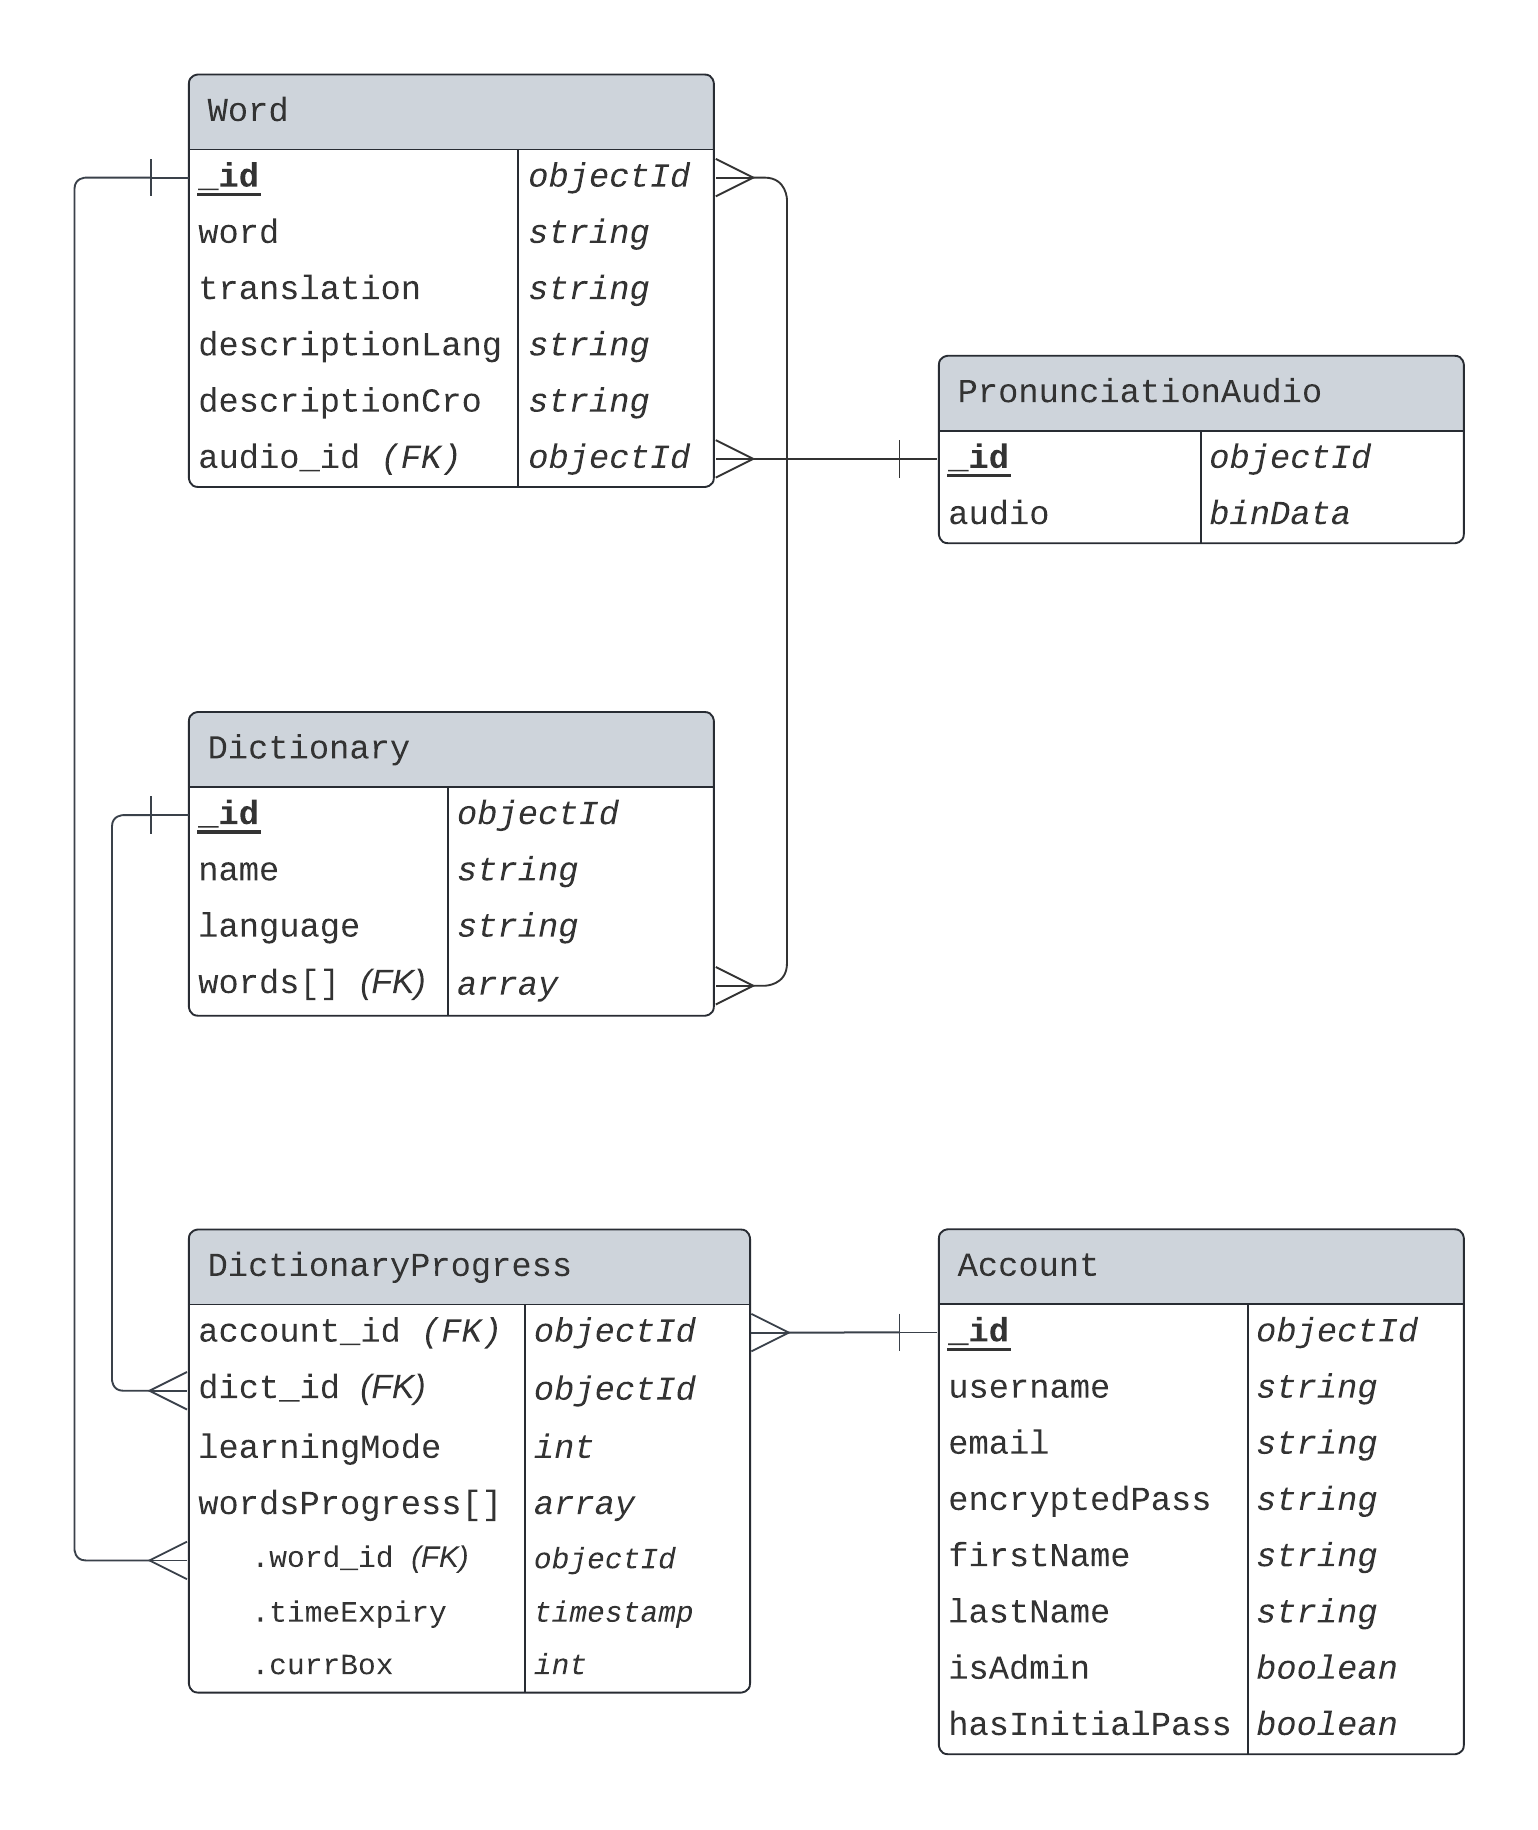
\includegraphics[width=\textwidth]{dijagrami/CanonPrinterDB.png} %veličina u odnosu na širinu linije
				\caption{Dijagram baze podataka}
				\label{fig:ER_dijagram} %label mora biti drugaciji za svaku sliku
			\end{figure}
			
			\eject
			
			
		\section{Dijagram razreda}

			\indent{Na slikama 4.3, 4.4 i 4.5 su prikazani razredi koji pripadaju {\textit{backend}} dijelu MVC (MTV)
			arhitekture. Razredi prikazani na slici 4.3 pirkazuju Controller razred. Metode implementirane u tim razredima
			manipuliraju s DTO razredima ({\textit{Data transfer object}}) koji služe za prijenos podataka između baze podataka i
			aplikacije. Atributi koji se nalaze u DTO razredima dohvaćaju se pomoću metoda implementiranih unutra Model razreda. 
			Metode implementirane unutar Controller razreda vraćaju JSON datoteke.}

			\indent{Zbog lakše oraganizacije, razredi su podijeljeni logički po pravu pristupa metodama određenih aktora. Kako
			bi se smanjila prenatrpanost unutar pojedinog dijagrama, prikazane su samo ovisnosti između razreda koji pripadaju
			istom dijelu dijagrama. Također se iz naziva i tipova atributa može zaključiti vrsta ovisnosti i povezanosti između
			različitih razreda.}

			\begin{figure}[H]
				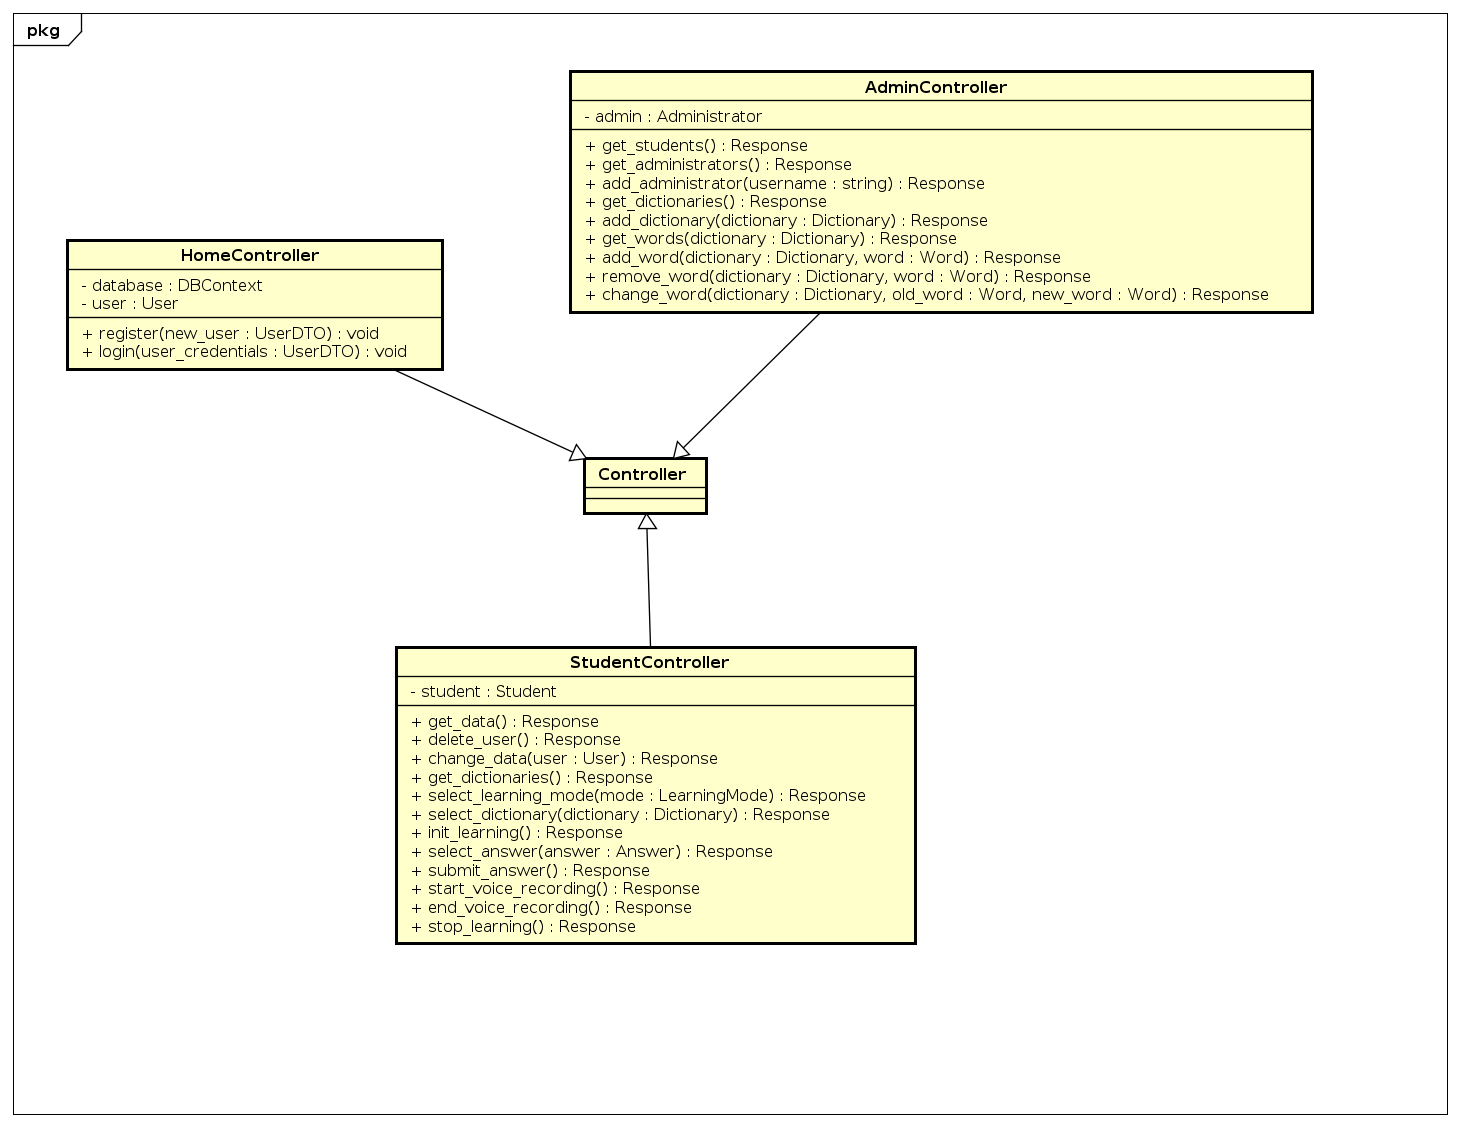
\includegraphics[width=\textwidth]{dijagrami/classcont.png} %veličina u odnosu na širinu linije
				\caption{Dijagram razreda - dio Controllers}
				\label{fig:classcont} %label mora biti drugaciji za svaku sliku
			\end{figure}

			\begin{figure}[H]
				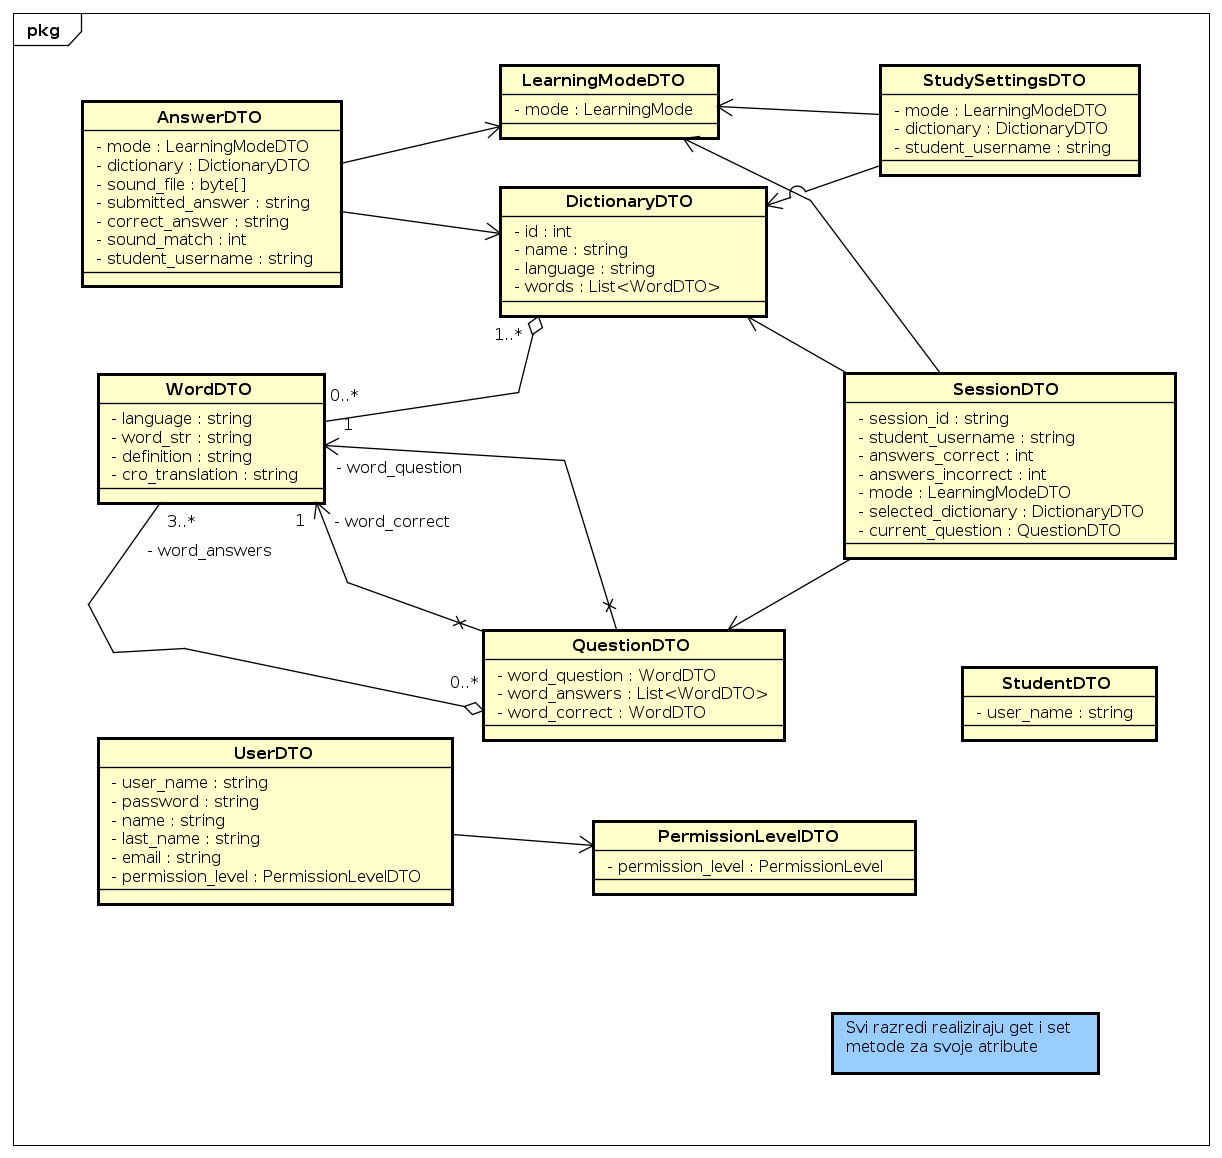
\includegraphics[width=\textwidth]{dijagrami/classdto.png} %veličina u odnosu na širinu linije
				\caption{Dijagram razreda - dio Data Transfer Objects}
				\label{fig:classdto} %label mora biti drugaciji za svaku sliku
			\end{figure}

			\indent{Model razredi zapravo preslikavaju strukturu baze podataka u aplikaciji. Implementirane metode direktno
			komuniciraju s bazom podataka i vraćaju tražene podatke. Razred CustomUser predstavlja korisnika koji se može
			registrirati u aplikaciju (ako nema već kreiran korisnički račun), ulogirati u aplikaciju, pregledavati i mijenjati
			svoje korisničke podatke te izbrisati svoj korisnički račun. Na razred CustomUser se vežu razredi Administrator i
			Student koji predstavljaju korisnike aplikacije. Razred CustomUser je također povezan s razredom PermissionLevel
			u kojem je zapisano koju razinu dozvole ima korisnik te se prema tome određuje je li korisnik Student ili Administrator.
			Razred Administrator je povezan s razredima Dictionary i Word jer administrator ima mogućnost uređivanja rječnika
			u aplikaciji. Razred Student je povezan s razredima Dictionary (student može odabrati rječnik za učenje), LearningMode
			(student odabire način učenja jezika) i s razredom Session. Razred Session predstavlja srž aplikacije, što je učenje
			stranog jezika. Povezan je s razredima Answer, Question i LearningMode, a preko tih razreda i s razredima Dictionary,
			Word itd. Taj razred služi za pohranu studentovog odgovora, pitanja, izgovora riječi, načina učenja... te u njemu
			student prekida svoje učenje.}

			\begin{figure}[H]
				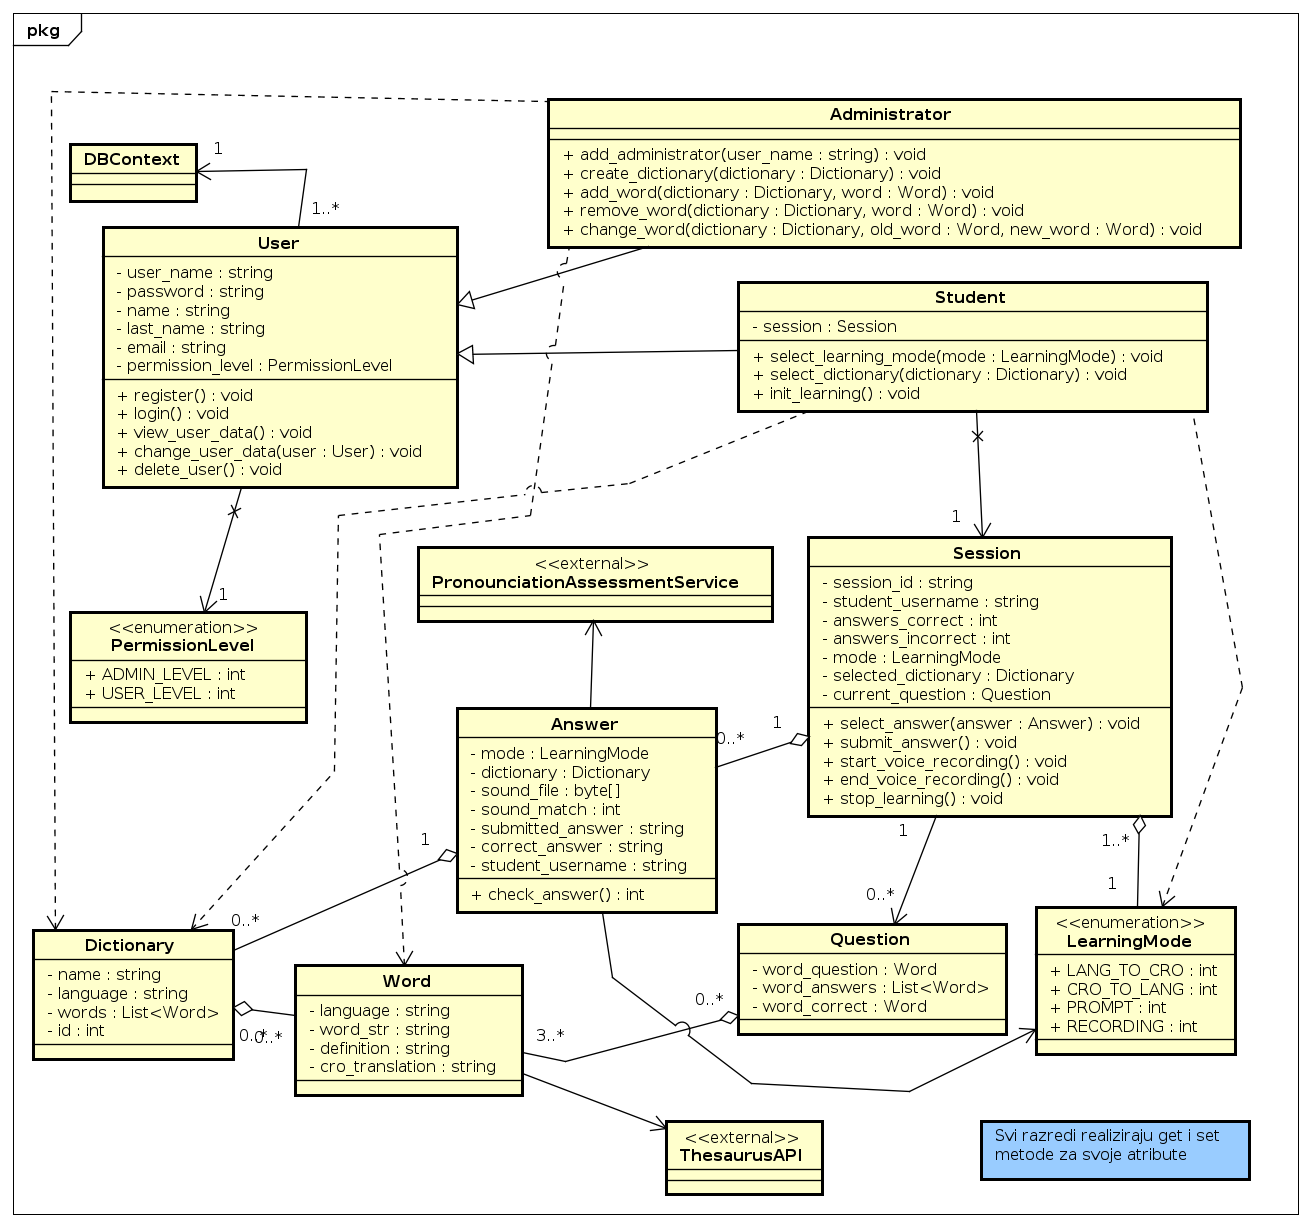
\includegraphics[width=\textwidth]{dijagrami/classmodel.png} %veličina u odnosu na širinu linije
				\caption{Dijagram razreda - dio Models}
				\label{fig:classmodel} %label mora biti drugaciji za svaku sliku
			\end{figure}
					
			
			\eject
		
		\section{Dijagram stanja}
			
			\noindent{Slika \ref{fig:Dijagram stanja učenika} prikazuje stanja kroz koje se može naći učenik koristeći aplikaciju.} \\
			\indent{Svakom korisniku prilikom posjeta aplikaciji se prikazuje uvodna stranica gdje se korisnik može, ukoliko već posjeduje račun, prijaviti pritiskom na tipku "Login" u gornjem desnom kutku prilikom čega će se od korisnika tražiti adresa e-pošte i lozinka. Nakon unosa te pritiskom na tiku Log in ispod unosa, ukoliko su vjerodajnice ispravne, korisnik će biti prijavljen. Ako korisnik ne posjeduje račun, moguće ga je registrati pritiskom na tipku "Sign up" u gornjem desnom kutku prilikom čega se od korisnika zahtjeva da upiše svoju adresu e-pošte na koju će se poslati inicijalna lozinka. Nakon unosa adrese e-pošte te pritiskom na tipku "Sign up" ispod unosa, korisnika se vraća na uvodnu stranicu gdje se može prijaviti s inicijalnom lozinkom dobivenu na adresu e-pošte. Nakon prve prijave od registracije, od korisnika se zahtjeva promjena inicijalne lozinke. Ovaj korak nije moguće zaobići i od korisnika će se zahtjevati promjena inicijalne lozinke prilikom svake prijave dok ju ne promijeni. } \\			\indent{Kada se učenik uspješno prijavi u sustav, prikazuje mu se učenička stranica na kojoj može nastaviti učiti rječnike, pregledavati sve rječnike, ažurirati podatke računa i odjaviti se. Dodantno, nakon svake prijave se u web-preglednik zapisiju kolačići vezani za prijavu tako da kada korisnik ponovno posjeti aplikaciju u istom web-pregledniku, biti će automatski prijavljen.} \\
			\indent{Da bi učenik započeo, ili nastavio, učenje nekog rječnika, potrebno ga je odabrati pritiskom na tipku "Customize learning" prilikom čega će se ponuditi opcija odabira jezika, a nakon odabira jezika ponudit će se svi rječnici na odabranom jeziku. Odabirom jednog od ponuđenih rječnika potrebno je još i odabrati načine učenja. Dostupna su 4 načina učenja: (1) upitom riječi iz rječnika uz odabir hrvatskog prijevoda: (2) upitom hrvatske riječi uz odabir prijevoda na jezik rječnika; (3) izgovorom riječi iz rječnika uz slovkanje riječi; (4) upitom riječi iz rječnika uz snimanje izgovora riječi. Svi načini učenja sastoje se od niza pitanja gdje se od učenika zahtjeva odabri točnog odgovora, točan izgovor ili točno slovkanje. Učenje se prekida pritiskom na tipku "FINISH" prilikom čega se učenika vraća na učeničku stranicu. } \\
			\indent{Na učeničkoj stranici moguće je i pregledati sve rječnike pritiskom na tipku "View dictionary" prilikom čega se od učenika traži jezik rječnika, a tek onda odabir rječnika na odabranom jeziku. Prikazati će se samo riječi iz rječinka bez prijevoda ili mogućnosti slušanja izgovora.} \\
			\indent{Učenik je u mogućnositi u svakom trenutku pregledati podatke svojeg računa i upravljati računom pritiskom na tipku "Profile" u gornjem  desnom kutku prilikom čega se učeniku prikazuje stranica za pregled i upravljanje računom. Ukoliko učenik želi promijeniti neki podatak, klikom na odgovrajuće polje može unijeti ažurirani podatak. Učenik može više podataka promijeniti odjednom, a svi promijenjeni podaci se ažuriraju tek nakon pritiska tipke "Save Changes". Važno je napomenuti da adresu e-pošte nije moguće promijeniti. Ukoliko učenik želi izbrisati račun, potrebno je pritisnuti tipku "Delete Account". Također je u svakom trenutku moguće odjaviti se čime se korisnika vraća na uvodnu stranica aplikacije, a kolačići za prijavu brišu tako da prilikom sljedećeg posjeta aplikaciji ne bude automatski prijavljen.}
			
			\begin{figure}[H]
				\centering
				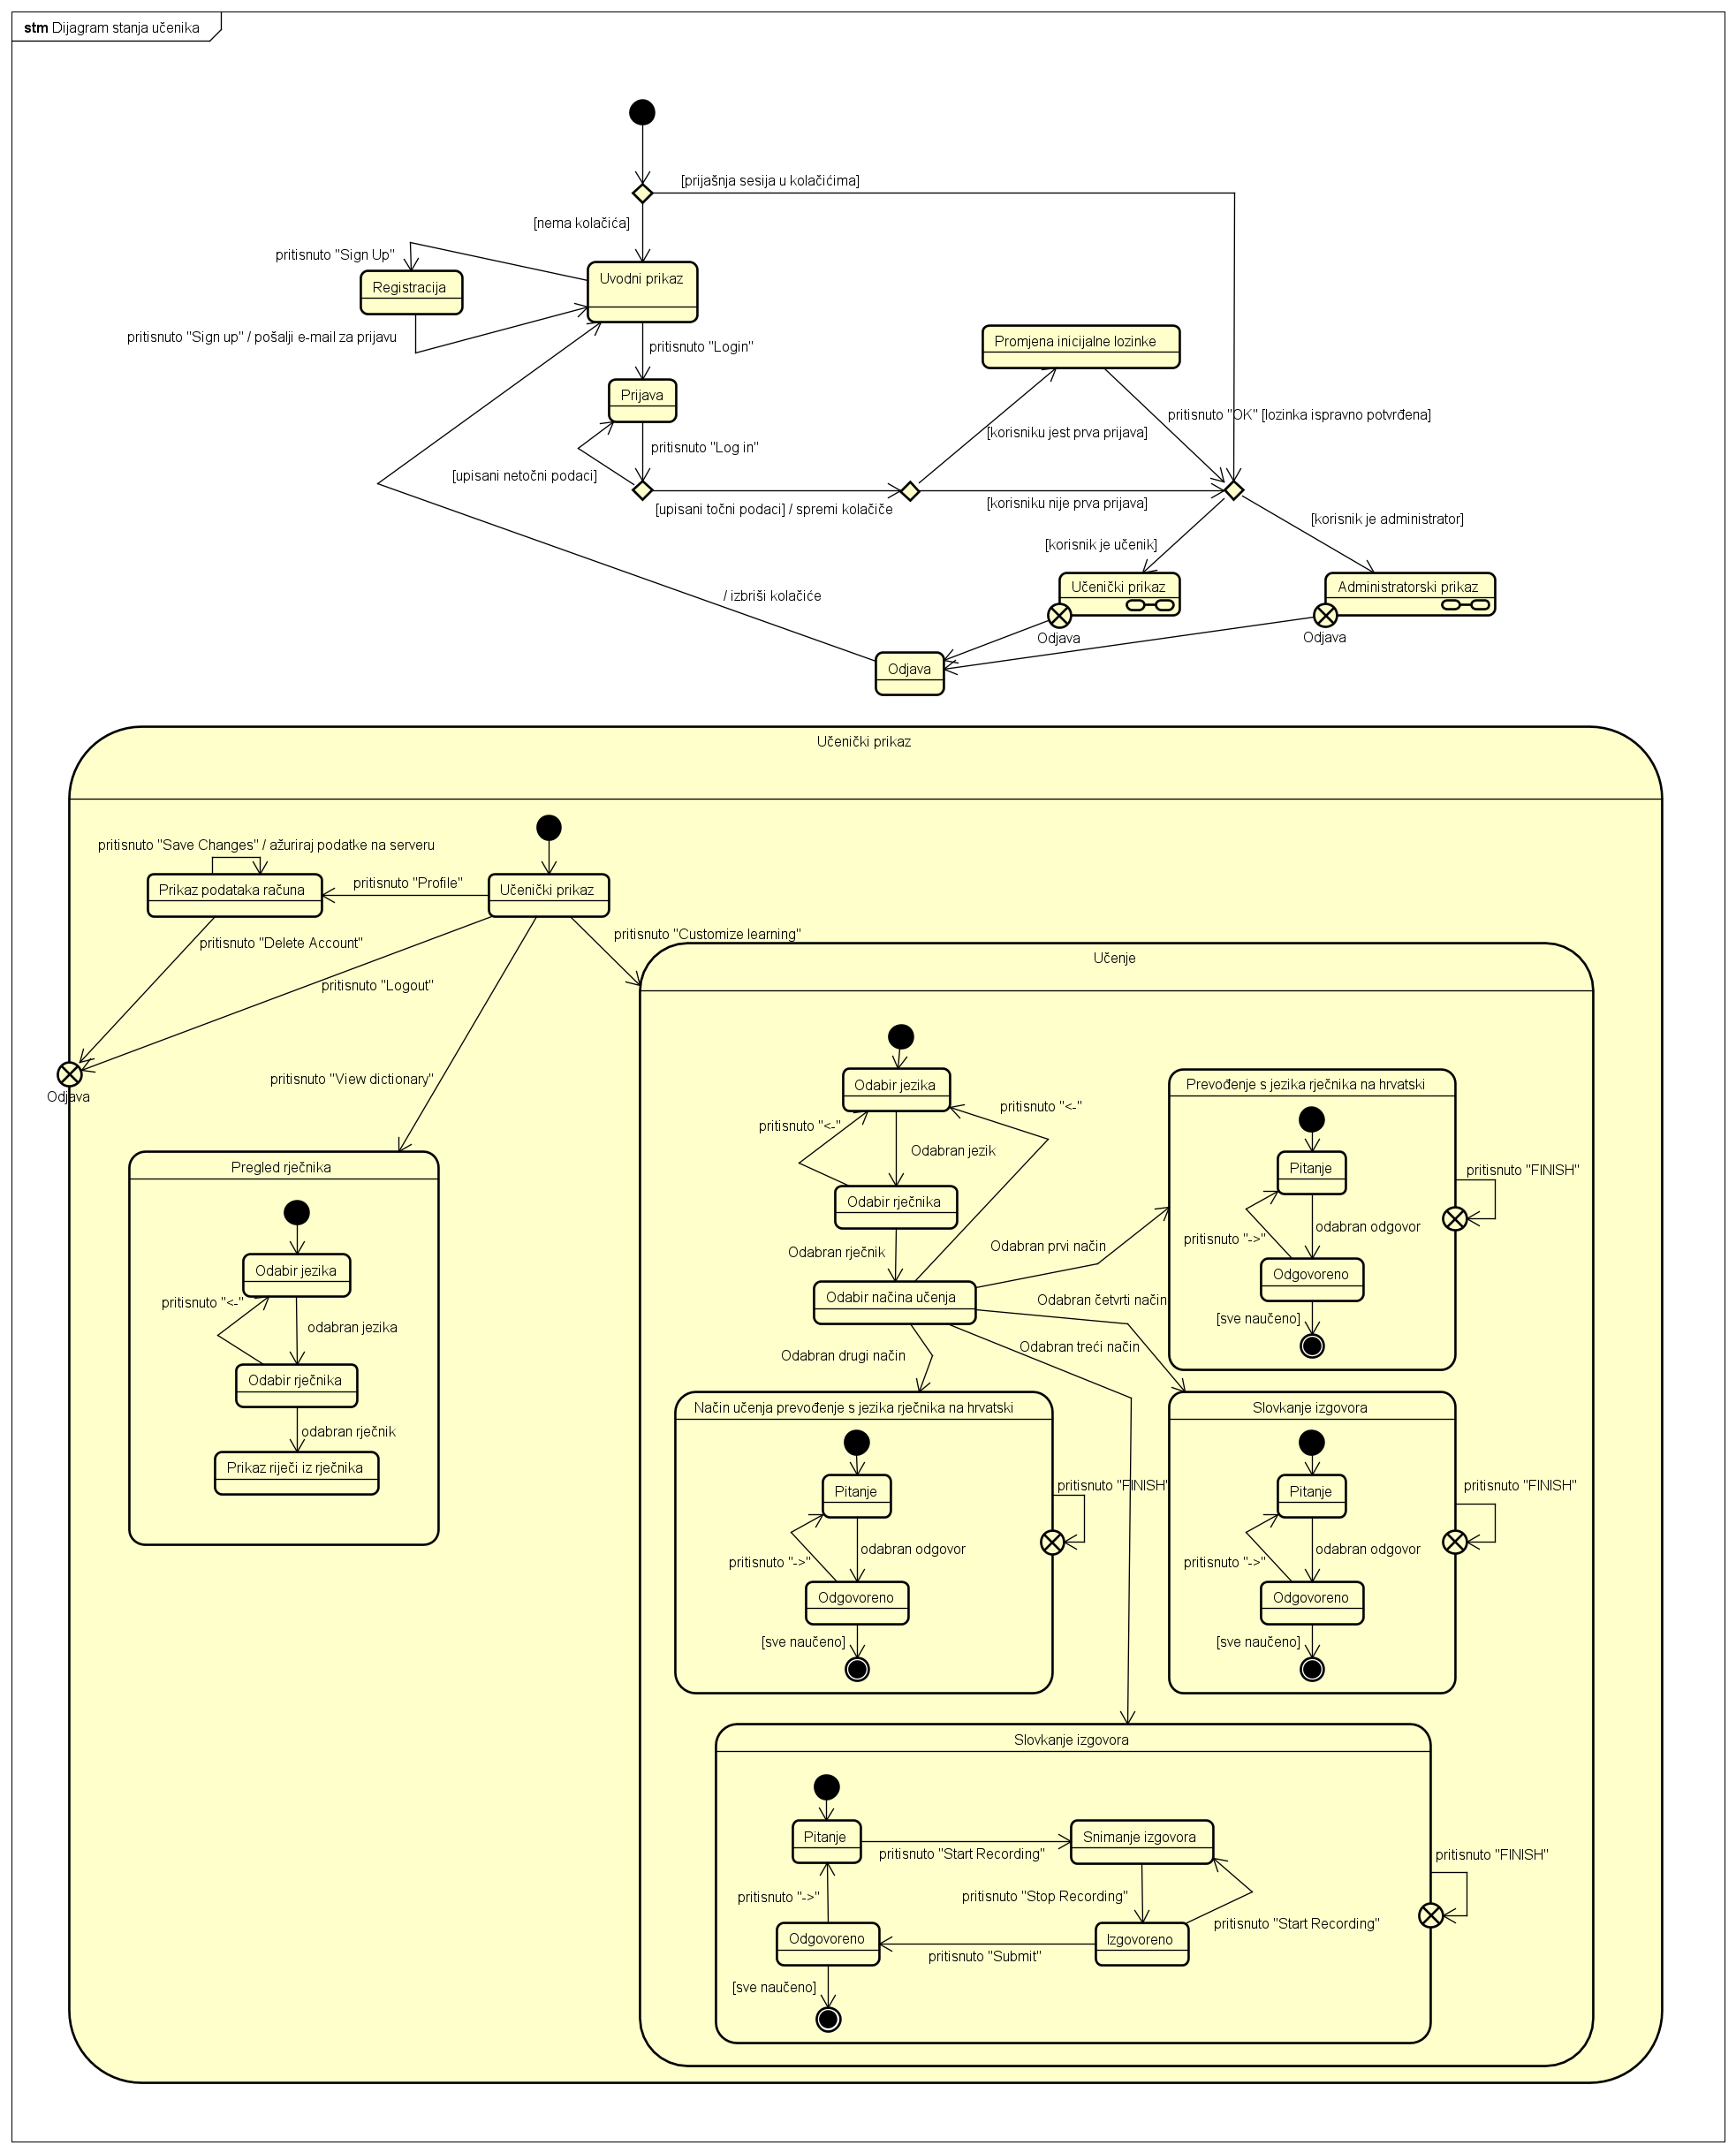
\includegraphics[width=\textwidth]{dijagrami/Dijagram_stanja_ucenika.png}
				\caption{Dijagram stanja učenika}
				\label{fig:Dijagram stanja učenika}
			\end{figure}
			
			
			\eject 
		
		\section{Dijagram aktivnosti}
		
			\noindent{Slika \ref{fig:Dijagram aktivnosti dodavanja nove riječi} prikazuje dijagram aktivnosti sustava kada administrator dodaje novu riječ.} \\
			\indent{Za dodavanje nove riječi administrator je dužan unjeti podatke o novoj riječi, a to su: vrsta riječi, sama riječ, opis riječi na jeziku rječnika, prijevod na hrvatski i riječnik kojem će riječ pripadati. Prilikom tipkanja same riječi, web-aplikacija će na svaku promjenu upisa regairati tako da predloži nekolicinu riječi na osnovi teksta koje je administrator do tada utipkao. Administrator tada može odabrati svoju riječ ako se nalazi u listi prijedloga, a ako ne, natipkati ju do kraja. Dodatno, kada administrator upiše riječ, web-aplikacija će automatski popuniti polje za opis riječi prikladnim opisom za tu riječ na osnovi vrste riječi. Administrator opis po volji može mijenjati.} \\
			\indent{Kada je administrator upisao sve potrebne podatke o novoj riječi, može pritisnuti gumb "Add word" prilikom čega će web-aplikacija slati zahtjev na server za dodaju nove riječi. Prije dodaje riječi, server u svojoj bazi podataka provjerava je li ista riječ već postoji u zadanom rječniku, ako postoji, ignorirat će zahtjev, a ako riječ ne postoji u rječniku, onda će ju uspješno dodati.}

			\begin{figure}[H]
				\centering
				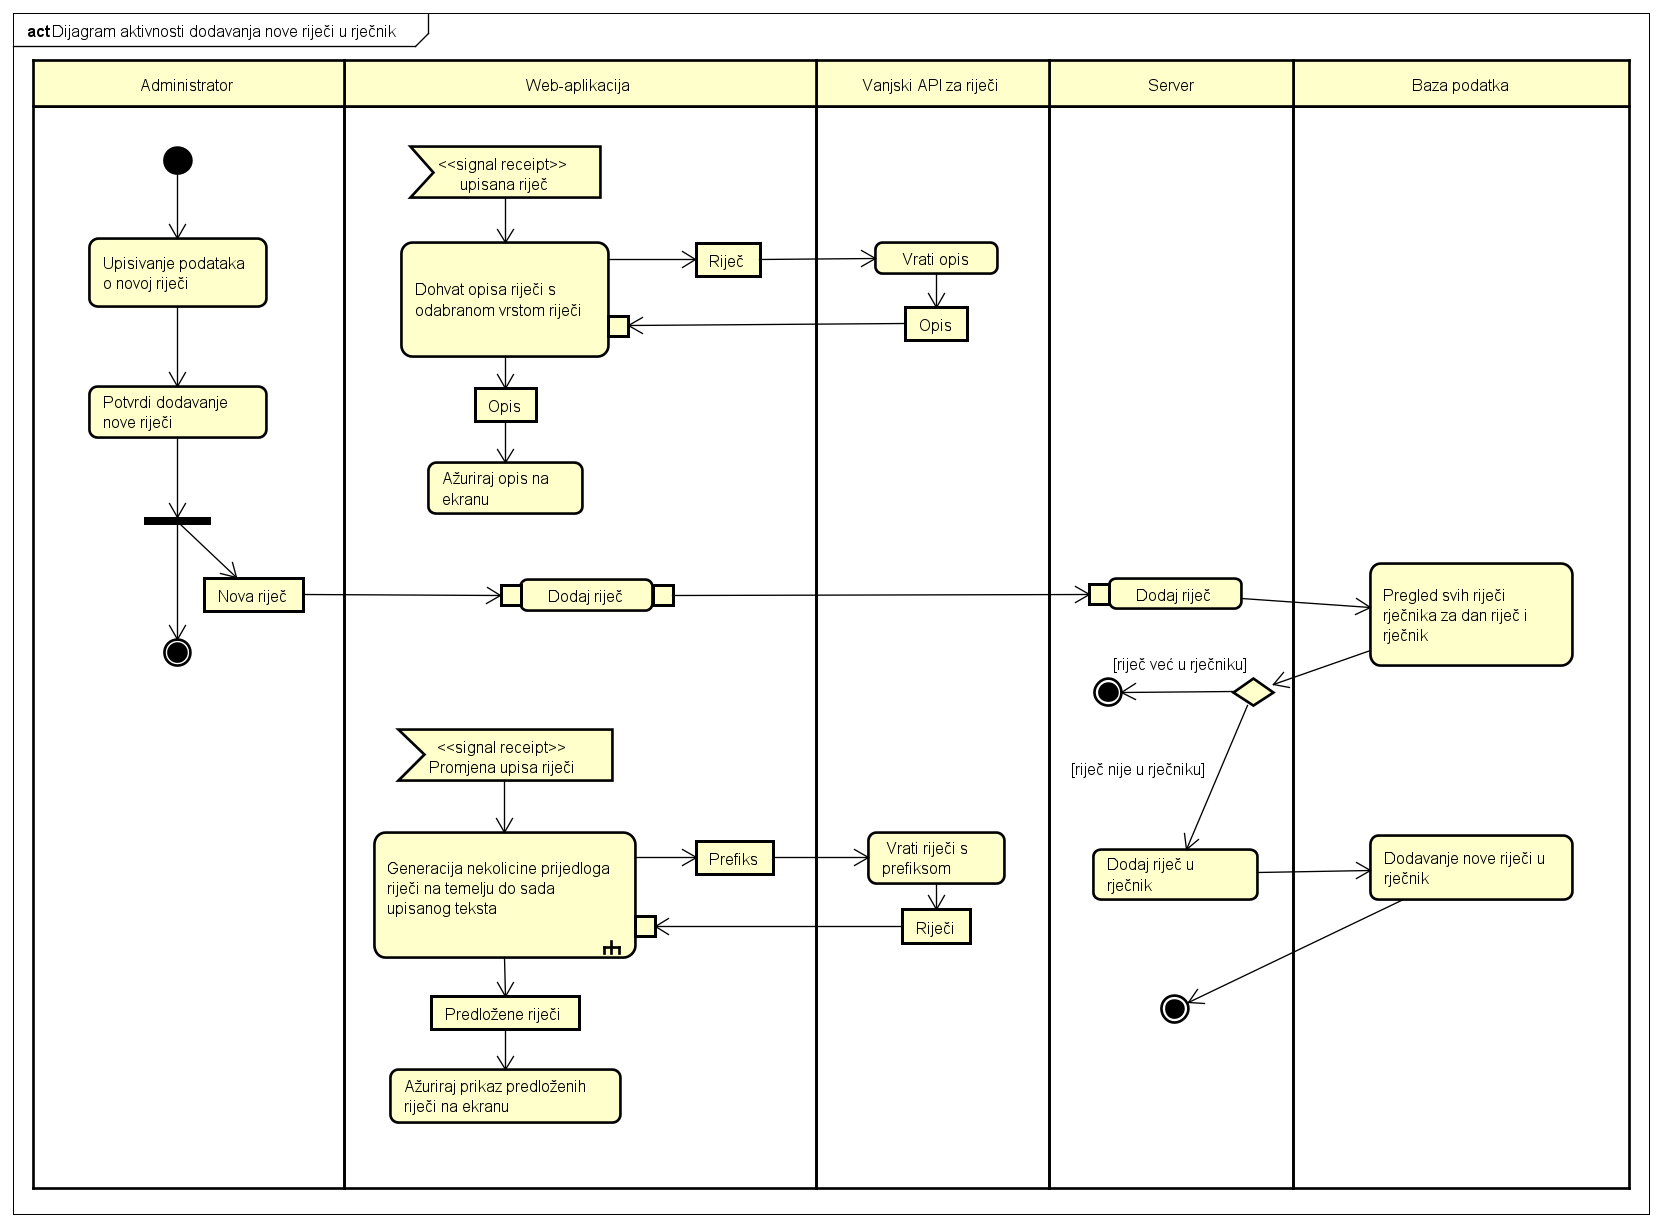
\includegraphics[width=\textwidth]{dijagrami/Dijagram_aktivnosti_dodavanja_nove_rijeci.png}
				\caption{Dijagram aktivnosti dodavanja nove riječi}
				\label{fig:Dijagram aktivnosti dodavanja nove riječi}
			\end{figure}
			
			\eject
		\section{Dijagram komponenti}
		
			\textbf{\textit{dio 2. revizije}}\\
		
			 \textit{Potrebno je priložiti dijagram komponenti s pripadajućim opisom. Dijagram komponenti treba prikazivati strukturu cijele aplikacije.}
	\chapter{Implementacija i korisničko sučelje}
		
		
		\section{Korištene tehnologije i alati}
			 
			 \noindent{Za izradu UML dijagrama korišten je alat Astah UML\footnote{\url{https://astah.net/products/astah-uml/}}}. Kao razvojno okruženje korišten je Visual Studio Code\footnote{\url{https://code.visualstudio.com/}}. Korišten je Git\footnote{\url{https://git-scm.com/}} kao sustav za upravljanje verzijama zajedno sa GitHub-om\footnote{\url{https://github.com/}} na kojem se nalazi udaljeni repozitorij projekta. Za potrebe izrade dokumentacije korišten je TeXstudio\footnote{\url{https://www.texstudio.org/}}, višeplatformski LaTeX editor otvorenog koda.\\
			 \indent{Za izradu backenda korišten je Django\footnote{\url{https://www.djangoproject.com/}}, besplatni radni okvir otvorenog koda za izradu web aplikacija u programskom jeziku Python\footnote{\url{https://www.python.org/}}. Za izradu frontenda korišten je React\footnote{\url{https://react.dev/}}, biblioteka napisana u programskom jeziku JavaScript\footnote{\url{https://developer.mozilla.org/en-US/docs/Web/JavaScript}}.}\\
			 \indent{Za potrebe baze podataka korišten je MongoDB\footnote{\url{https://www.mongodb.com/}}. Sama baza podataka nalazi se na udaljenom poslužitelju. Usluga koja omogućuje pristup, rad i postavljanje udaljene MongoDB baze podataka je MongoDB Atlas\footnote{\url{https://www.mongodb.com/atlas/database}}. Aplikacija je puštena u pogon na udaljenom poslužitelju pomoću usluge koje nudi Heroku\footnote{\url{https://www.heroku.com/}}. Heroku je cloud platforma kao usluga koja omogućuje puštanje u pogon aplikacija i podržava više programskih jezika.}\\
			 \indent{Za potrebe komunikacije tima korištene su aplikacije WhatsApp\footnote{\url{https://www.whatsapp.com/}} i Microsoft Teams\footnote{\url{https://www.microsoft.com/en-us/microsoft-teams/group-chat-software}}.
			 Za potrebe testiranja aplikacije osim ugrađene potpore za testiranje koju nudi Django korišten je i Selenium WebDriver\footnote{\url{https://www.selenium.dev/documentation/webdriver/}} koji omogućuje pisanje i automatizaciju testova za web aplikacije.}
			 
			
			
			\eject 
		
	
		\section{Ispitivanje programskog rješenja}
			
			\textbf{\textit{dio 2. revizije}}\\
			
			 \textit{U ovom poglavlju je potrebno opisati provedbu ispitivanja implementiranih funkcionalnosti na razini komponenti i na razini cijelog sustava s prikazom odabranih ispitnih slučajeva. Studenti trebaju ispitati temeljnu funkcionalnost i rubne uvjete.}
	
			
			\subsection{Ispitivanje komponenti}
			\textit{Potrebno je provesti ispitivanje jedinica (engl. unit testing) nad razredima koji implementiraju temeljne funkcionalnosti. Razraditi \textbf{minimalno 6 ispitnih slučajeva} u kojima će se ispitati redovni slučajevi, rubni uvjeti te izazivanje pogreške (engl. exception throwing). Poželjno je stvoriti i ispitni slučaj koji koristi funkcionalnosti koje nisu implementirane. Potrebno je priložiti izvorni kôd svih ispitnih slučajeva te prikaz rezultata izvođenja ispita u razvojnom okruženju (prolaz/pad ispita). }
			
			
			
			\subsection{Ispitivanje sustava}
			
			 \textit{Potrebno je provesti i opisati ispitivanje sustava koristeći radni okvir Selenium\footnote{\url{https://www.seleniumhq.org/}}. Razraditi \textbf{minimalno 4 ispitna slučaja} u kojima će se ispitati redovni slučajevi, rubni uvjeti te poziv funkcionalnosti koja nije implementirana/izaziva pogrešku kako bi se vidjelo na koji način sustav reagira kada nešto nije u potpunosti ostvareno. Ispitni slučaj se treba sastojati od ulaza (npr. korisničko ime i lozinka), očekivanog izlaza ili rezultata, koraka ispitivanja i dobivenog izlaza ili rezultata.\\ }
			 
			 \textit{Izradu ispitnih slučajeva pomoću radnog okvira Selenium moguće je provesti pomoću jednog od sljedeća dva alata:}
			 \begin{itemize}
			 	\item \textit{dodatak za preglednik \textbf{Selenium IDE} - snimanje korisnikovih akcija radi automatskog ponavljanja ispita	}
			 	\item \textit{\textbf{Selenium WebDriver} - podrška za pisanje ispita u jezicima Java, C\#, PHP koristeći posebno programsko sučelje.}
			 \end{itemize}
		 	\textit{Detalji o korištenju alata Selenium bit će prikazani na posebnom predavanju tijekom semestra.}
			
			\eject 
		
		
		\section{Dijagram razmještaja}
			
			\noindent{Na dijagramu razmještaja je prikazana topologija sustava i odnos programskih artefakata.}
			
			\indent{Web aplikacija se kao programski artefakt izvršava u Heroku Dyno spremniku koji je vrsta Linux spremnika proširen sa raznim mogućnostima upravljanja koje nudi Heroku platforma.}
			
			\indent{Aplikacija ovisi o bazi podataka koja se nalazi na MongoDB Atlas poslužitelju. Pristup i rad s bazom podataka omogućuje usluga MongoDB Atlas Cluster. Za potrebe dohvata podataka o riječima aplikacija koristi Datamuse API.}
			
			\indent{Korisnici (učenici i administratori riječi) koriste web preglednik kako bi pristupili web aplikaciji. Arhitektura sustava bazira se na arhitekturi "klijent - poslužitelj". Komunikacija između korisničkog računala i poslužitelja odvija se preko HTTPS veze.}
			
			\begin{figure}[H]
				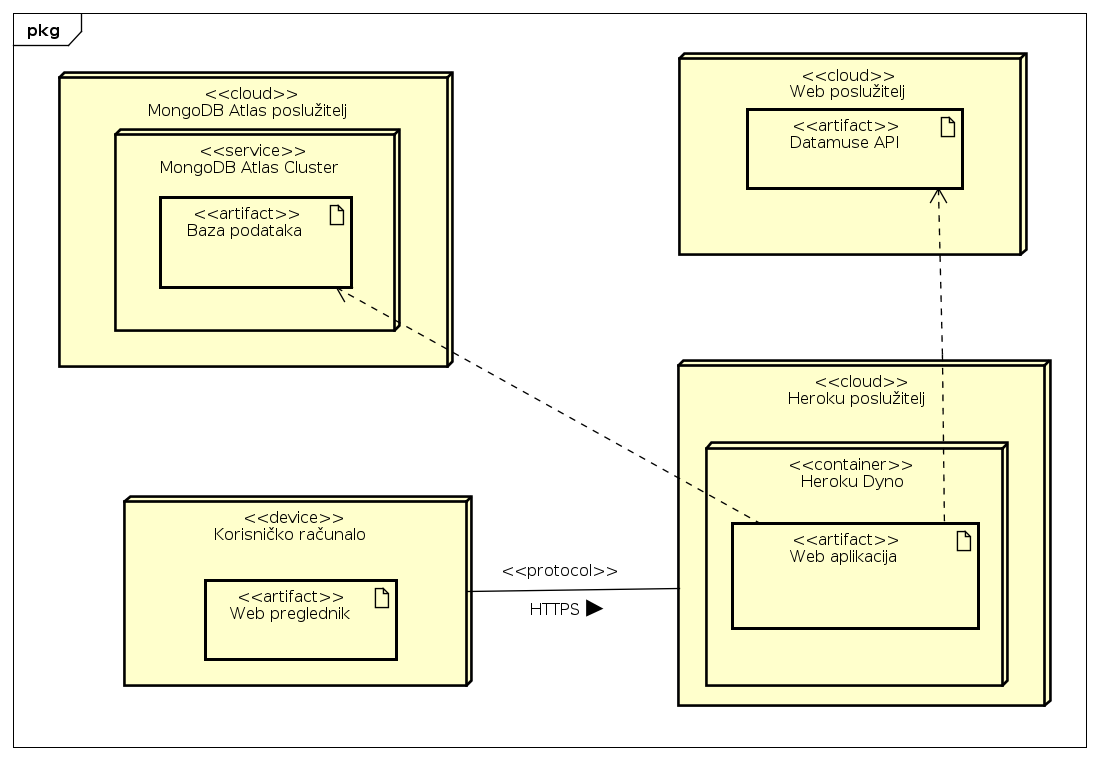
\includegraphics[width=\textwidth]{dijagrami/dijagram_razmjestaja.png} %veličina u odnosu na širinu linije
				\caption{Dijagram razmještaja}
				\label{fig:Dijagram_razmjestaja} %label mora biti drugaciji za svaku sliku
			\end{figure}
			
			\eject 
		
		\section{Upute za puštanje u pogon}
			
			\noindent{\textbf{Konfiguracija poslužitelja baze podataka}}\\
			
			\noindent{\textbf{Konfiguracija baze podataka}}\\
			
			\noindent{\textbf{Konfiguracija Heroku poslužitelja}}\\
			\noindent{Nakon što se uspješno izradi Heroku korisnički račun, potrebno je stvoriti novu aplikaciju u "Dashboardu" klikom na "Create new app". Potrebno je upisati ime aplikacije, odabrati regiju i završiti stvaranje aplikacije klikom na "Create app". Forma za izradu aplikacije je prikazana na slici \ref{fig:StvaranjeAplikacije}}.
			
			
			\begin{figure}[H]
				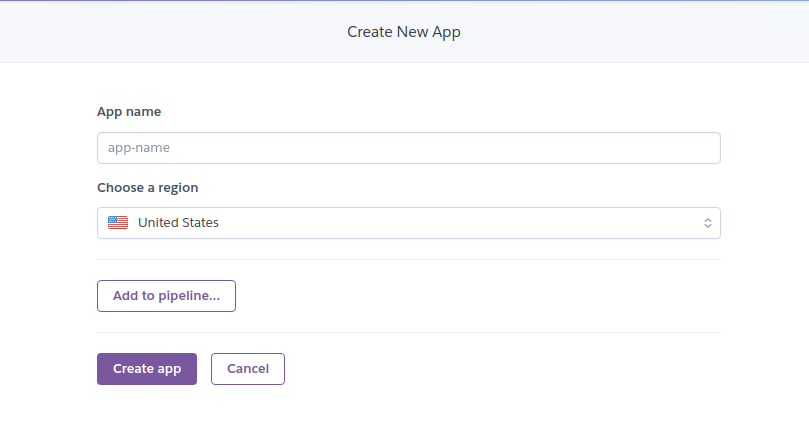
\includegraphics[width=\textwidth]{slike/stvaranjeAplikacije.png} %veličina u odnosu na širinu linije
				\caption{Stvaranje nove aplikacije}
				\label{fig:StvaranjeAplikacije} %label mora biti drugaciji za svaku sliku
			\end{figure}
		
			
			\indent{Nakon izrade aplikacije potrebno je podesiti konfiguraciju u "Settings" dijelu aplikacije kao što je prikazano na slikama \ref{fig:podesi1} i \ref{fig:podesi2}. "DB CONNECTION STRING" se dobije prilikom konfiguracije baze podataka i služi aplikaciji za pristup bazi podataka, a "SECRET KEY" je tajni ključ čija će vrijednost ovisiti o konkretnom projektu, Django ga interno koristi za potrebe hashiranja. Moguće je i podesiti ostale parametre po potrebi.}\\
			\indent{Potrebno je i dodati "Buildpack" za Node.js i Python s obzirom da aplikacija koristi programski jezik Python za backend, a React za frontend. "Buildpackovi" služe za instaliranje svega onoga što je potrebno da bi se aplikacija mogla pokrenuti na Heroku poslužitelju.}
			
			
			\begin{figure}[H]
				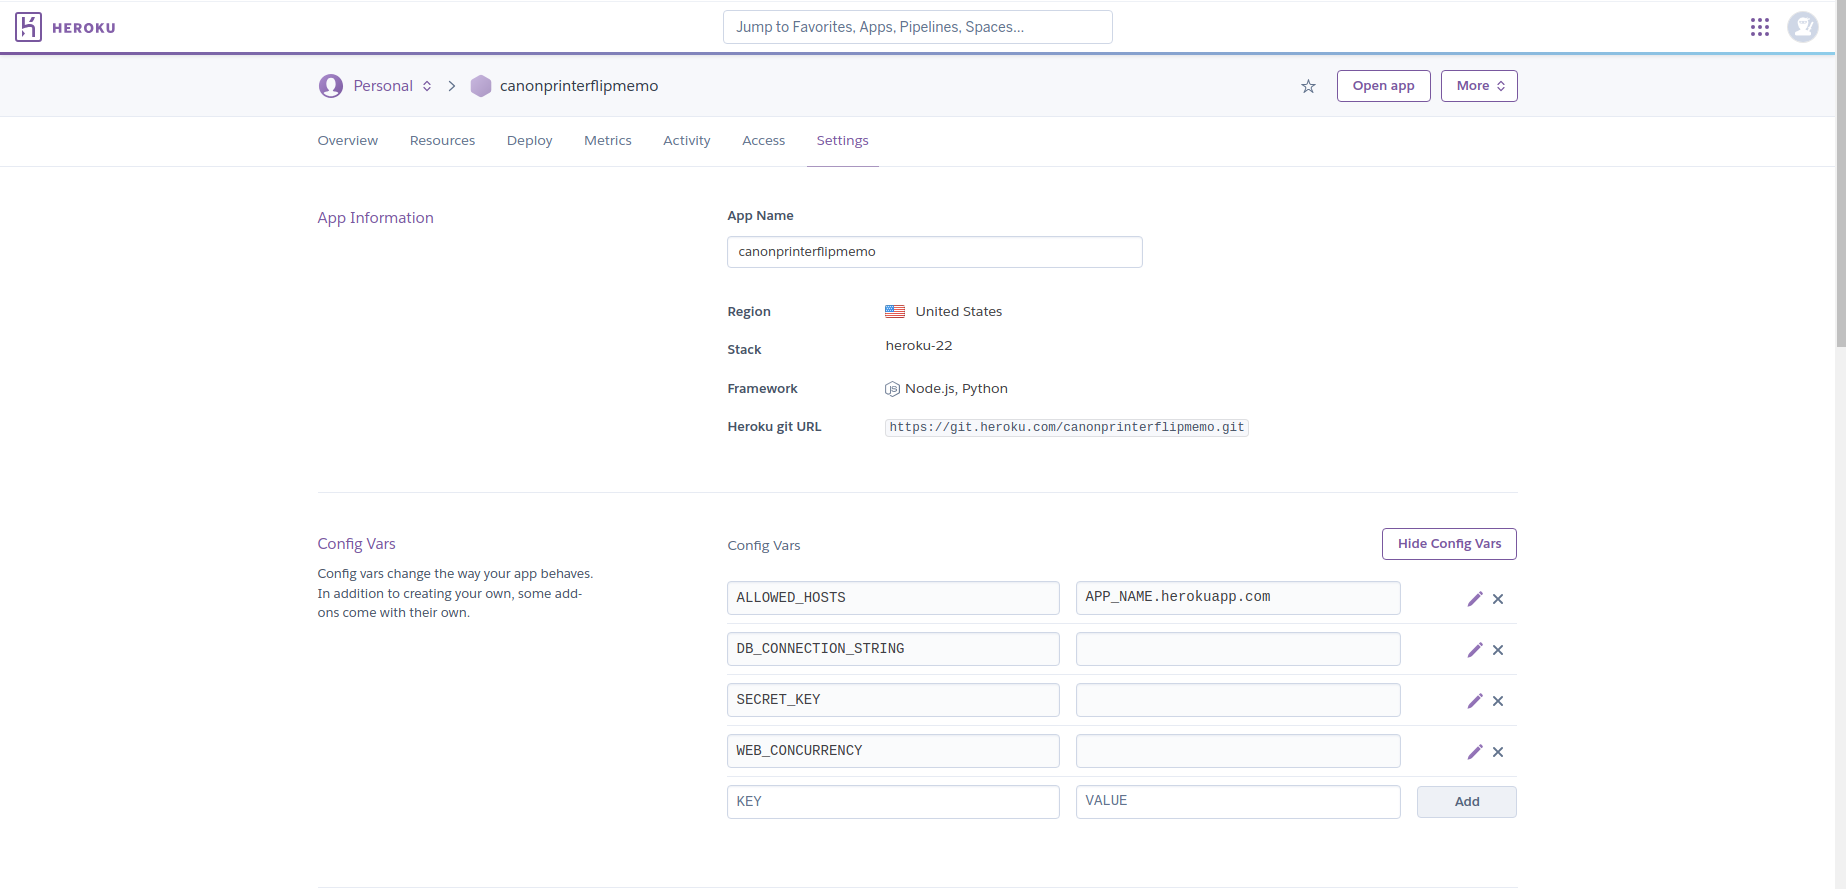
\includegraphics[width=\textwidth]{slike/podesi1.png} %veličina u odnosu na širinu linije
				\caption{Konfiguracija konfiguracijski varijabli}
				\label{fig:podesi1} %label mora biti drugaciji za svaku sliku
			\end{figure}
		
			\begin{figure}[H]
				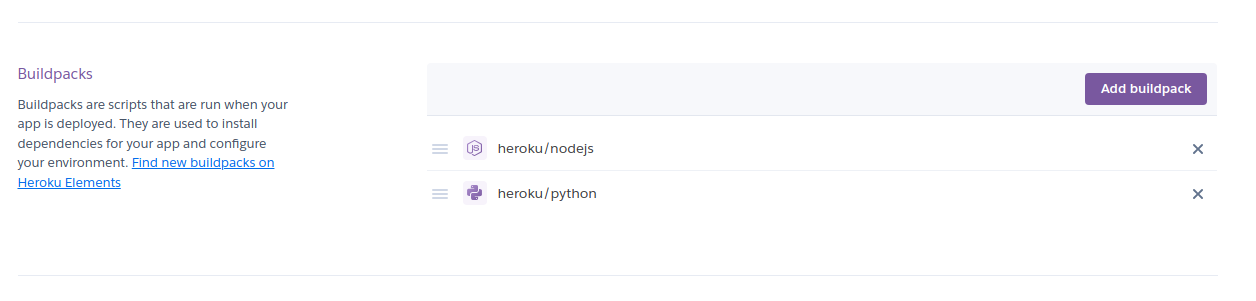
\includegraphics[width=\textwidth]{slike/podesi2.png} %veličina u odnosu na širinu linije
				\caption{Konfiguracija "Buildpackova"}
				\label{fig:podesi2} %label mora biti drugaciji za svaku sliku
			\end{figure}
		
			\noindent{\textbf{Organizacija strukture projekta za puštanje u pogon}}\\
			\noindent{Za potrebe puštanje aplikacije u pogon pomoću Heroku usluge, potrebno je organizirati strukturu projekta odnosno izvornog koda u onakvu strukturu kakvu Heroku očekuje prilikom prijenosa izvornog koda na Heroku poslužitelj. Reorganizacija strukture projekta većim dijelom uključuje reorganizaciju postojeće hijerarhije direktorija, no potrebno je dodati i neke konfiguracijske datoteke što je opisano u nastavku.}\\
			\indent{Na slici \ref{fig:organizacijaKoda} je prikazan primjer strukture projekta kakvu očekuje Heroku. "FlipMemo", "main" i "users" su mape iz Django dijela aplikacije, a "src", "public" iz React dijela aplikacije. Bitno je da sve te mape budu na istoj razini u glavnom direktoriju "CanonPrinter". "staticfiles" mapa je trenutno prazna, no u nju se prilikom puštanja u pogon spremaju razne datoteke nakon što se odradi "build" na Heroku poslužitelju.}
			
			\begin{figure}[H]
				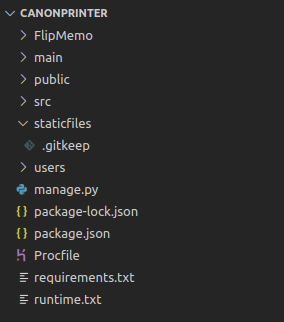
\includegraphics[width=\textwidth]{slike/organizacijaKoda.png} %veličina u odnosu na širinu linije
				\caption{Struktura projekta za puštanje aplikacije u pogon}
				\label{fig:organizacijaKoda} %label mora biti drugaciji za svaku sliku
			\end{figure}
		
			\noindent{"manage.py", "package.json" i "package-lock.json" su datoteke koje postoje i prije reorganizacije strukture projekta, a vezanu su uz Django i React dok su "Procfile", "requirements.txt" i "runtime.txt" konfiguracijske datoteke koje Heroku očekuje da postoje u projektu i moraju se dodati prije puštanja aplikacije u pogon. Sadržaj konfiguracijskih datoteke prikazan je na slikama \ref{fig:konf1}, \ref{fig:konf2}, \ref{fig:konf3}. 
			
			\begin{figure}[H]
				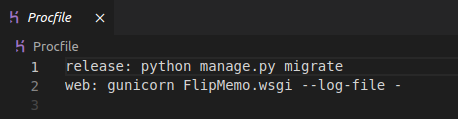
\includegraphics[width=\textwidth]{slike/konf1.png} %veličina u odnosu na širinu linije
				\caption{Procfile}
				\label{fig:konf1} %label mora biti drugaciji za svaku sliku
			\end{figure}
		
			\begin{figure}[H]
				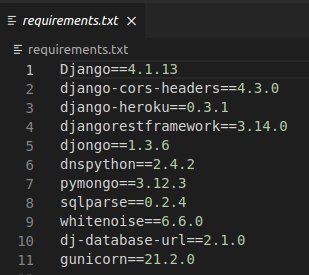
\includegraphics[width=\textwidth]{slike/konf2.png} 	%veličina u odnosu na širinu linije
				\caption{requirements.txt}
				\label{fig:konf2} %label mora biti drugaciji za svaku sliku
			\end{figure}
		
			Svaka konfiguracijska datoteka sadrži konfiguracijske parametre koji su potrebni prilikom puštanja aplikacije u pogon, npr. verzije svih potrebnih biblioteka koje je potrebno instalirati, verziju programskog jezika Python i sl. Za detalje o tome kako Heroku koristi te konfiguracijske datoteke upućujemo na službenu dokumentaciju\footnote{\url{https://devcenter.heroku.com/categories/reference}}.}
	
			\begin{figure}[H]
				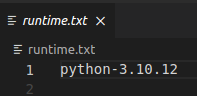
\includegraphics[width=\textwidth]{slike/konf3.png} %veličina u odnosu na širinu linije
				\caption{runtime.txt}
				\label{fig:konf3} %label mora biti drugaciji za svaku sliku
			\end{figure}
		
			\noindent{\textbf{Puštanje aplikacije u pogon korištenjem Heroku Git}}\\
			\noindent{Nakon provedenih svih potrebnih prethodno opisanih koraka, aplikacije se može pustiti u pogon na Heroku poslužitelj na više načina. Ovdje prikazujemo način puštanja aplikacije u pogon korištenjem Heroku Gita. Potrebno je instalirati Heroku CLI koji omogućuje rad sa Heroku korištenjem komandne linije \footnote{\url{https://devcenter.heroku.com/articles/heroku-cli}}.}\\
			\indent{Nakon što je Heroku CLI uspješno instaliran za odgovarajuću platformu, potrebno je provesti postupak prijenosa izvornog koda projekta na Heroku poslužitelj kojim se automatski pokreće i proces izgradnje i puštanja aplikacije u pogon. Slika \ref{fig:herokucli} prikazuje sve potrebne korake kod rada sa Heroku CLI. Aplikacija je nakon provedenih koraka dostupna na poveznici koju je izgenerirao proces puštanja aplikacije u pogon. Moguće je i zadati svoju vlastitu domenu na kojoj će aplikacija biti dostupna što je prikazano na slici \ref{fig:customDomena}}.
			
			\begin{figure}[H]
				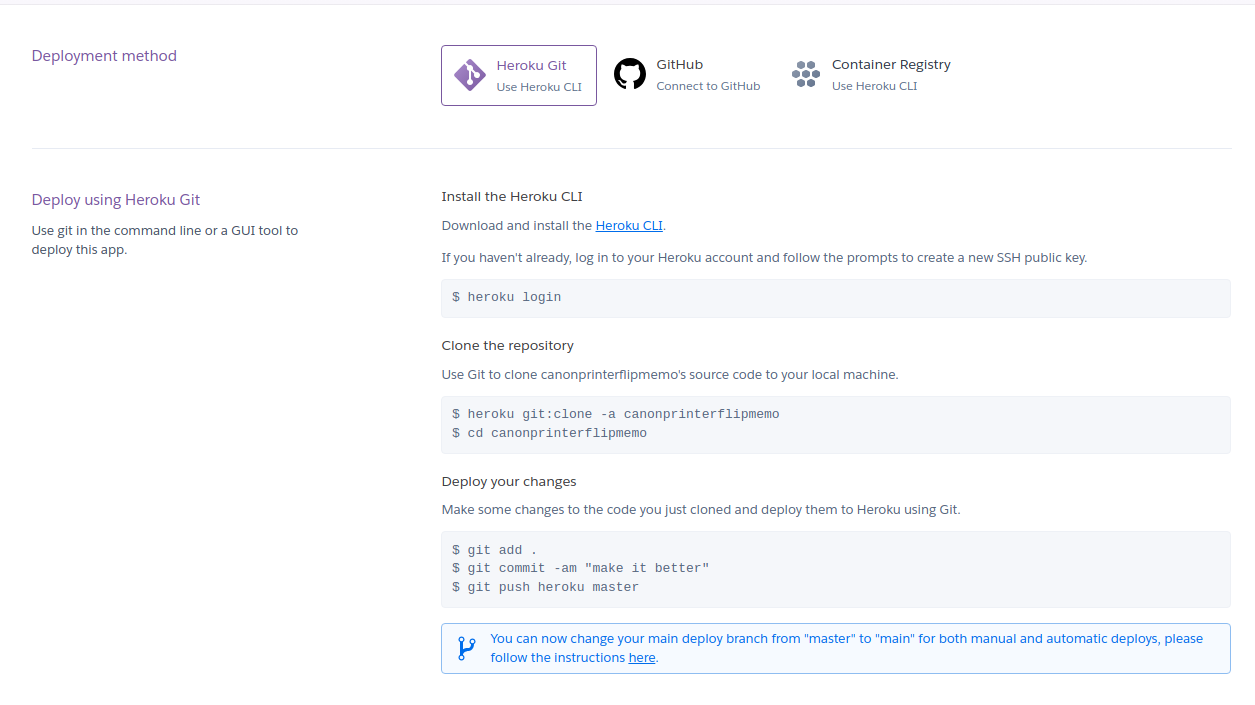
\includegraphics[width=\textwidth]{slike/herokucli.png} %veličina u odnosu na širinu linije
				\caption{Puštanje aplikacije u u pogon korištenjem Heroku CLI}
				\label{fig:herokucli} %label mora biti drugaciji za svaku sliku
			\end{figure}
		
			\begin{figure}[H]
				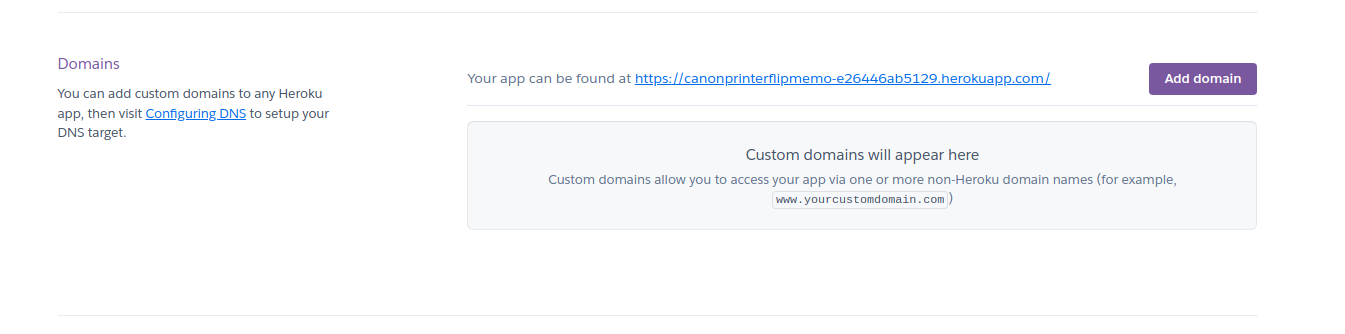
\includegraphics[width=\textwidth]{slike/customDomena.png} %veličina u odnosu na širinu linije
				\caption{Dio postavka za podešavanje domene aplikacije}
				\label{fig:customDomena} %label mora biti drugaciji za svaku sliku
			\end{figure}
			
			\eject 
	\chapter{Zaključak i budući rad}
		
		 \noindent{Zadatak naše grupe je bio razvoj web aplikacije za učenje stranih jezika na osnovu ponavljanja s odmakom ( eng. spaced repetition). Aplikacija u sebi ima podržana čak 4 različita moda učenja, opciju dodavanja/brisanja i uređivanja riječi/rječnika. Aplikacija je u potpunosti napravljena nakon 14 tjedana te je odrađena prema uputama i prema samom tekstu zadatka. Projekt je bio podijeljen u dvije faze.}
		
		 \indent{Prva faza projekta se sastojala od okupljanja tima, podjele zadataka/dužnosti te rada na opsežnoj dokumentaciji. Kvalitetna priprema i izrada dokumentacije u velikoj je mjeri olakšala kasniji rad na funkcionalnostima same aplikacije. Izrada obrazaca i dijagrama je jedan od najvažnijih dijelova dokumentacije. Dobro razrađeni obrasci uporabe, sekvencijski dijagrami, model baze podataka, dijagram razreda su bili od velike koristi frontend i backend podtimovima koji su prema njima razvijali funkcionalnosti aplikacije. Virtualni prikazi idejnih rješenja su riješili većinu nedoumica backend i frontend timova tijekom druge faze odnosno implementiranja funkcionalnosti te dovođenju aplikacije u „život“. }

		 \indent{Druga faza je natjerala sve članove tima da ubace u petu brzinu. Zbog kraćeg vremenskog roka, veće količine posla kojeg je trebalo odraditi te manjak iskustva u radu na „velikim„ projektima radilo se punom parom. Manjak znanja i iskustva u izradi je članove tima primorao na proučavanje prethodno odabranih tehnologija te brušenje do sada stečenog znanja u sklopu obrazovanja. Osim same implementacije funkcionalnosti trebalo je još i izraditi popratnu dokumentaciju te sitno modificirati prethodno napravljenu dokumentaciju u prvoj fazi izrade projekta. Temeljita i detaljna izrada dokumentacije u prvoj fazi projekta je omogućila laku modifikaciju te značajno smanjila rizik od vremenski skupih ispravaka na implementaciji funkcionalnosti.}

		 \indent{Komunikacija članova grupe se odvijala putem alata Whatsapp i Teams. Svi članovi tima su bili jako dobro upućeni u napredak izrade projekta zbog kvalitetno izabranih alata. Aplikacija se još mogla dodatno proširiti dodavanjem podrške za mobilne telefone te eventualnom izradom prave aplikacije koja bi imala mogućnost skidanja na uređaj za razliku od web aplikacije kojoj se može pristupiti samo uz pomoć web preglednika.}

		 \indent{Samo sudjelovanje na ovako dugotrajnom i opsežnom projektu je bilo vrijedno za svakog člana tima. Uz redovite obaveze smo iskusili kako je raditi na pravom velikom projektu s ograničenim vremenskim rokom isporuke i intenzivnim radom koji zadatak zahtijeva. Ključni faktor ovog projekta bila je dobra organiziranost članova tima te dobro vodstvo samog tima.  Bez obzira na veliki prostor za usavršavanje smo zadovoljni odrađenim poslom te će nam ovo znanje i iskustvo puno pomoći u daljnjem usavršavanju vještina. }
		
		\eject 
	\chapter*{Popis literature}
		\addcontentsline{toc}{chapter}{Popis literature}
	 	
 		\textbf{\textit{Kontinuirano osvježavanje}}
	
		\textit{Popisati sve reference i literaturu koja je pomogla pri ostvarivanju projekta.}
		
		
		\begin{enumerate}
			
			
			\item  Programsko inženjerstvo, FER ZEMRIS, \url{http://www.fer.hr/predmet/proinz}
			
			\item  I. Sommerville, "Software engineering", 8th ed, Addison Wesley, 2007.
			
			\item  T.C.Lethbridge, R.Langaniere, "Object-Oriented Software Engineering", 2nd ed. McGraw-Hill, 2005.
			
			\item  I. Marsic, Software engineering book``, Department of Electrical and Computer Engineering, Rutgers University, \url{http://www.ece.rutgers.edu/~marsic/books/SE}
			
			\item  The Unified Modeling Language, \url{https://www.uml-diagrams.org/}
			
			\item  Astah Community, \url{http://astah.net/editions/uml-new}
		\end{enumerate}
		
		 
	
	
	\begingroup
	\renewcommand*\listfigurename{Indeks slika i dijagrama}
	%\renewcommand*\listtablename{Indeks tablica}
	%\let\clearpage\relax
	\listoffigures
	%\vspace{10mm}
	%\listoftables
	\endgroup
	\addcontentsline{toc}{chapter}{Indeks slika i dijagrama}


	
	\eject 
		
	\chapter*{Dodatak: Prikaz aktivnosti grupe}
		\addcontentsline{toc}{chapter}{Dodatak: Prikaz aktivnosti grupe}
		
		\section*{Dnevnik sastajanja}
		
		
		\begin{packed_enum}
			\item  sastanak
			
			\item[] \begin{packed_item}
				\item Datum: 24. listopada 2023.
				\item Prisustvovali: Jurica Runtas, Lovro Švenda, Josip Ćurić,
				Matej Galić, Jan Kuzman, Kristijan Milić
				\item Teme sastanka:
				\begin{packed_item}
					\item  odabir alata i tehnologija
					\item  podjela poslova vezanih uz razradu specifikacije programske potpore i dokumentiranje zahtjeva
				\end{packed_item}
			\end{packed_item}
		
			\item sastanak
			\item[] \begin{packed_item}
			\item Datum: 31. listopada 2023.
			\item Prisustvovali: Jurica Runtas, Lovro Švenda, Josip Ćurić,
			Matej Galić, Jan Kuzman, Kristijan Milić
			\item Teme sastanka:
			\begin{packed_item}
				\item  podjela poslova vezanih uz razradu arhitekture sustava, baze podataka i dijagrama razreda
			\end{packed_item}
			\end{packed_item}
	
			\item sastanak
			\item[] \begin{packed_item}
			\item Datum: 8. studenoga 2023.
			\item Prisustvovali: Jurica Runtas, Lovro Švenda, Josip Ćurić,
			Matej Galić, Jan Kuzman, Kristijan Milić
			\item Teme sastanka:
			\begin{packed_item}
				\item dogovor i raspodjela poslova vezanih uz implementaciju generičkih funkcionalnosti
				\item rasprava oko izgleda i dizajna aplikacije
				\item detalji oko implementacije i povezivanja baze podataka sa aplikacijom
			\end{packed_item}
			\end{packed_item}
			
		\end{packed_enum}
		
		\eject
		\section*{Tablica aktivnosti}
		
			\textbf{\textit{Kontinuirano osvježavanje}}\\
			
			 \textit{Napomena: Doprinose u aktivnostima treba navesti u satima po članovima grupe po aktivnosti.}

			\begin{longtblr}[
					label=none,
				]{
					vlines,hlines,
					width = \textwidth,
					colspec={X[7, l]X[1, c]X[1, c]X[1, c]X[1, c]X[1, c]X[1, c]X[1, c]}, 
					vline{1} = {1}{text=\clap{}},
					hline{1} = {1}{text=\clap{}},
					rowhead = 1,
				} 
			
				\SetCell[c=1]{c}{} & \SetCell[c=1]{c}{\rotatebox{90}{\textbf{Jurica Runtas }}} & \SetCell[c=1]{c}{\rotatebox{90}{\textbf{Matej Galić }}} &	\SetCell[c=1]{c}{\rotatebox{90}{\textbf{Jan Kuzman }}} & \SetCell[c=1]{c}{\rotatebox{90}{\textbf{Lovro Švenda }}} &	\SetCell[c=1]{c}{\rotatebox{90}{\textbf{Kristijan Milić }}} & \SetCell[c=1]{c}{\rotatebox{90}{\textbf{Josip Ćurić }}} &	\SetCell[c=1]{c}{\rotatebox{90}{\textbf{Marin Bošković }}} \\  
				Upravljanje projektom 		& 4 &  &  &  &  &  & \\ 
				Opis projektnog zadatka 	&  &  & 3.5 &  &  &  & \\ 
				
				Funkcionalni zahtjevi       & 1 &  &  &  &  &  &  \\ 
				Opis pojedinih obrazaca 	& 1.5 &  &  & 3.5 & 1 &  &  \\ 
				Dijagram obrazaca 			&  &  &  &  & 3 &  &  \\ 
				Sekvencijski dijagrami 		&  & 4 &  &  &  & 3.5 &  \\ 
				Opis ostalih zahtjeva 		&  &  & 1 &  &  &  &  \\ 

				Arhitektura i dizajn sustava	 &  &  &  & 2.5 &  &  &  \\ 
				Baza podataka				&  &  &  &  &  & 4.5 &   \\ 
				Dijagram razreda 			& 1.5 &  &  &  & 3 &  &   \\ 
				Dijagram stanja				&  &  &  &  &  &  &  \\ 
				Dijagram aktivnosti 		&  &  &  &  &  &  &  \\ 
				Dijagram komponenti			&  &  &  &  &  &  &  \\ 
				Korištene tehnologije i alati 		&  &  &  &  &  &  &  \\ 
				Ispitivanje programskog rješenja 	&  &  &  &  &  &  &  \\ 
				Dijagram razmještaja			&  &  &  &  &  &  &  \\ 
				Upute za puštanje u pogon 		&  &  &  &  &  &  &  \\  
				Dnevnik sastajanja 			&  &  &  &  &  &  &  \\ 
				Zaključak i budući rad 		&  &  &  &  &  &  &  \\  
				Popis literature 			&  &  &  &  &  &  &  \\  
				&  &  &  &  &  &  &  \\ \hline 
				\textit{Izrada backenda za generičke funkcionalnosti} 			&  &  &  & 15 & 2 &  &  \\ 
				\textit{Dodatne stavke kako ste podijelili izradu aplikacije} 			&  &  &  &  &  &  &  \\ 
				\textit{npr. izrada početne stranice} 				&  &  &  &  &  &  &  \\  
				\textit{izrada baze podataka} 		 			&  &  &  &  &  & 1 & \\  
				\textit{spajanje s bazom podataka} 							&  &  &  &  &  & 5 &  \\ 
				\textit{back end} 							&  &  &  &  &  &  &  \\  
				 							&  &  &  &  &  &  &\\ 
			\end{longtblr}
					
					
		\eject
		\section*{Dijagrami pregleda promjena}
		
		\textbf{\textit{dio 2. revizije}}\\
		
		\textit{Prenijeti dijagram pregleda promjena nad datotekama projekta. Potrebno je na kraju projekta generirane grafove s gitlaba prenijeti u ovo poglavlje dokumentacije. Dijagrami za vlastiti projekt se mogu preuzeti s gitlab.com stranice, u izborniku Repository, pritiskom na stavku Contributors.}
		
	


\end{document} %naredbe i tekst nakon ove naredbe ne ulaze u izgrađen dokument 


